\documentclass{article}
% LaTex packages 
\usepackage[utf8]{inputenc}
\usepackage{amsfonts}
\usepackage{amsmath}
\usepackage{amsthm}
\usepackage{tabto}
\usepackage{booktabs}
\usepackage{hyperref}
\usepackage{xspace}
\usepackage[utf8]{inputenc}
\usepackage{fancyvrb}
\usepackage{stmaryrd}
\usepackage{graphicx}
\usepackage{url}
\usepackage[onehalfspacing]{setspace}
% Theorems
\usepackage{pgf}
\usepackage{tikz}
\usetikzlibrary{arrows}
\usepackage{graphicx}
\usepackage{setspace}
\usepackage{amssymb}
\usepackage{mathtools}
\usepackage{tabto}
\usepackage[T1]{fontenc}
\usepackage[a4paper,left=2cm,right=2cm,top=2cm,bottom=3cm]{geometry}
\usepackage{geometry}
 \geometry{
 a4paper,
 %total={170mm,257mm},
 %left=20mm,
 top=30mm,
 }

\newtheorem{thm}{Theorem}[section]
\newtheorem{cor}[thm]{Corollary}
\newtheorem{lem}[thm]{Lemma}
\newtheorem{prop}[thm]{Proposition}
\theoremstyle{definition}
\newtheorem{defn}[thm]{Definition}
\theoremstyle{remark}
\newtheorem{rem}[thm]{Remark}
\DeclarePairedDelimiter\ceil{\lceil}{\rceil}
\DeclarePairedDelimiter\floor{\lfloor}{\rfloor}
\newcommand{\eg}{e.g.,\xspace}
\newcommand{\encrypt}[1]{\ensuremath{E(#1)}\xspace}
\newcommand{\decrypt}[1]{\ensuremath{D(#1)}\xspace}

\renewcommand{\labelitemi}{$\bullet$}
\renewcommand{\labelitemii}{$\circ$}
\renewcommand{\labelitemiii}{$\cdot$}
\renewcommand{\labelitemiv}{$\ast$}

\usepackage{wrapfig}
\usepackage[font=small,labelfont=bf]{caption}

% ---- Bibliography ----

\usepackage{biblatex}
% \addbibresource{references.bib}
%------------------------------------
\begin{document}
\title{Summary ''Actionable Gamification - Beyond Points, Badges and Leaderboards''}
\author{\vspace{-2.0cm} Nicola Lea Libera}
\date{June 2020}
\maketitle

This is a summary of the book Yu-Kai Chou, \textit{''Actionable Gamification - Beyond Points, Badges and Leaderboards''}, 2014, Octalysis Media, USA.

\tableofcontents

\newpage

\section{Chapter 1: When the Surreal Blends into our World}
\subsection{Why Gamification?}
\begin{itemize}
    \item ''One of the earlier works done on adapting gameplay practices within the workplace can be traced back to 1984, when Charles Coonradt explored the value of adding game-play elements at work through his book ''The Game of Work''. \cite{game_work} \\
    Coonradt addressed the question, ''Why would people pay for the privilege of working harder at their chosen sport or recreational pursuit than they would work at a job where they were beeing paid?'' He then boiled it down to five conclusions that lead to hobbies being more preferable to work.
    \begin{itemize}
        \item Clearly defined goals
        \item Better scorekeeping and scorecards
        \item More frequent feedback
        \item A higher degree of personal choice of methods
        \item Consistent coaching''
    \end{itemize}
\end{itemize}

\subsection{Human-Focused Design: The Better Term for Gamification}
\begin{itemize}
    \item ''Human-Focused Design optimizes for human motivation in a system as opposed to optimizing for pure functional efficiency within the system
\end{itemize}

\subsection{The Conquests of Gamification}
\begin{itemize}
    \item In a few short years, gamification has reached a social tipping point and is starting to creep into every aspect of our lives - from education, work, marketing, parenting, sustainability, all the way to healthcare and scientific research:
    \begin{itemize}
        \item The U.S. Armed Forces now spends more money on recruitment games than any other marketing platform
        \item Volkswagen generated 33 million web visits and 119,000 new ideas through it's People Car Project to design the ''perfect car''.''
    \end{itemize}
    There are quite some more examples. A list can be found at \url{https://yukaichou.com/gamification-examples/} and stats can be found at \url{https://yukaichou.com/gamification-examples/gamification-stats-figures/}.
    \item ''According to the Entertainment Software Association, 70\% of major employers are already using gamification to enhance performance and training at their companies.''
    \item In a similar report, the market research firm Gartner predicted that 70\% of Fortune 500 firms would use Gamification by the end of 2014.''
    \item ''Unfortunately, in the same report, Gartner also predicted that 80\% of those gamified efforts will fail due to bad design[...].''
\end{itemize}

\newpage

\section{Chapter 2: The PBL Fallacy}
\subsection{Secondhand Sushi Making}
\begin{itemize}
    \item ''If you ask any gamer what makes a game fun, they will not tell you that it is because of the PBLs [(Points, Badges, Leaderboards]. They play it because there are elements of strategy and great ways to spend time with friends, or they want to challenge themselves to overcome difficult obstacles, depending on the context. This is the difference between extrinsic motivation, where you are engaged because of a goal or reward, and intrinsicmotivation, where the activity itself is fun and exciting, with or without a reward.''
\end{itemize}


\subsection{A Trojan Horse without Greek Soldiers}
\begin{itemize}
    \item ''Generic game mechanics and poorly construced game elements such as levels, boss fights or quests often fall into the same hole as PBLs. Simply put, applying traditional ''game elements'' ubiquitos in poular gameplay without diving deeper into user motivation contributes to shallow user experience [..].''
    \item Games aren't necessarily fun because of high quality graphics or flashy animations either. There are many unpoular, poor-selling games with state-of-the-art 3D high-resolution graphics.[..] Clearly, there are more to games than ''meets the eye''.
\end{itemize}

\subsection{The Story of the Good Designer vs. Bad Designer}
\begin{itemize}
    \item ''[..] a game might have all the ''right game elements'' but still be increadibly boring or stupid if they do not focus on theis users' motivation first.''
    \item Instead of starting with what game elements and game mechanics to use, the good game designer may begin by thinking ''Okay, how to I want my users to feel? Do I want them to feel inspired? Do I want them to feel proud? Should they be scared? Anxious? What's my goal for their intended experience?\\
    Once the designer understands how she wants her users to feel, then she begins to think, ''Okay, what kind of elements and mechanics can help me accomplish my goals of ensuring players feel this way.'' 
\end{itemize}

\newpage

\section{Chapter 3: The Octalysis Framework}
\begin{itemize}
    \item ''I saw that almost every successful game appeals to certain Core Drives within us and motivates us towards a variety of decisions and activities. I also noticed that different types of game techniques push us toward differently[..]. I drilled down to find what differentiates one type of motivation from another. The end result is a gamification design framework called Octalysis, which derives its name from an octagonal shape with 8 Core Drives representing each side.
    \begin{center}
            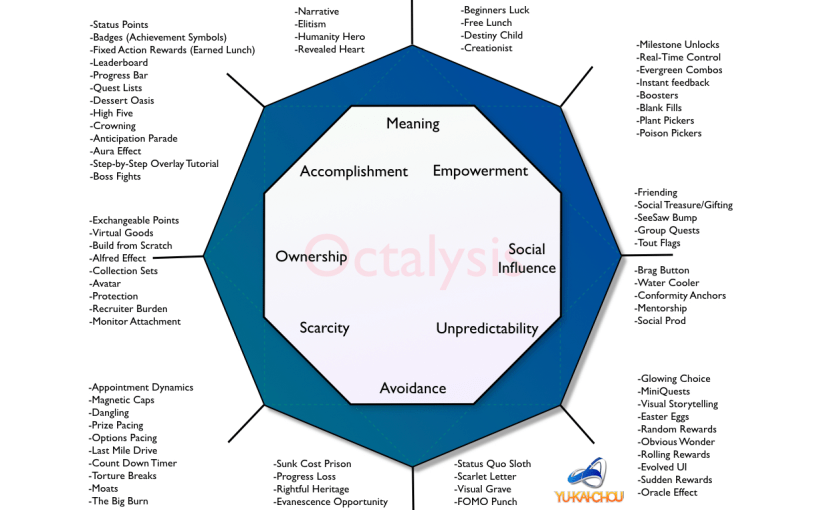
\includegraphics[width= 0.6\textwidth]{images/octaysis-gamification-framework.png}
    \end{center}
\end{itemize}

\subsection{The 8 Cor Drives of Gamification}
The following explanations are from Yu-Kai Chou's block (\url{https://yukaichou.com/gamification-examples/octalysis-complete-gamification-framework/}) and are more or less the same as described in his book.
\begin{itemize}
    \item \textbf{Core Drive 1: Epic Meaning \& Calling}
    \begin{center}
        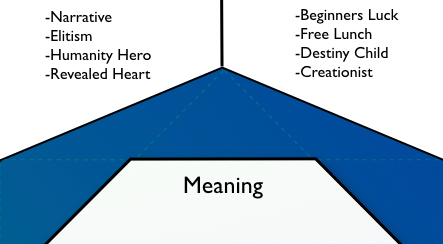
\includegraphics[width= 0.3\textwidth]{images/core-drive-1-epic-meaning-and-calling.png}
    \end{center}
    Epic Meaning \& Calling is the Core Drive where a player believes that he is doing something greater than himself or he was “chosen” to do something. A symptom of this is a player that devotes a lot of his time to maintaining a forum or helping to create things for the entire community (think Wikipedia or Open Source projects). This also comes into play when someone has “Beginner’s Luck” – an effect where people believe they have some type of gift that others don’t or believe they were “lucky” to get that amazing sword at the very beginning of the game.
    
    \item \textbf{Core Drive 2: Development \& Accomplishment}
    \begin{center}
        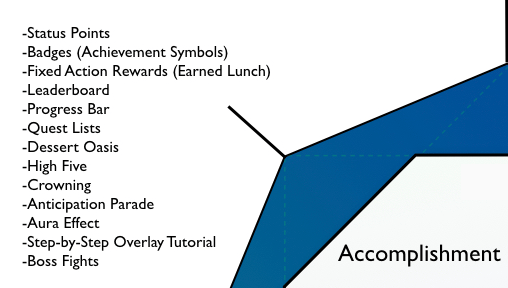
\includegraphics[width= 0.3\textwidth]{images/core-drive-2-development-and-accomplishment.png}
    \end{center}
    Development \& Accomplishment is the internal drive of making progress, developing skills, and eventually overcoming challenges. The word “challenge” here is very important, as a badge or trophy without a challenge is not meaningful at all. This is also the core drive that is the easiest to design for and coincidently is where most of the PBLs: points, badges, leaderboards mostly focus on.
    
    \item \textbf{Core Drive 3: Empowerment of Creativity \& Feedback}
    \begin{center}
        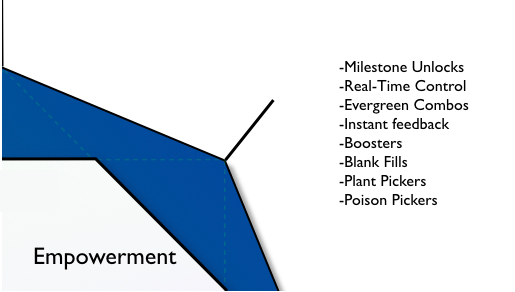
\includegraphics[width= 0.3\textwidth]{images/core-drive-3-empowerment-of-creativith-and-feedback.png}
    \end{center}
  Empowerment of Creativity \& Feedback is when users are engaged in a creative process where they have to repeatedly figure things out and try different combinations. People not only need ways to express their creativity, but they need to be able to see the results of their creativity, receive feedback, and respond in turn. This is why playing with Legos and painting are fun in-and-of themselves and often become Evergreen Mechanics, where a game-designer no longer needs to continuously add more content to keep the activity fresh and engaging.
  
      \item \textbf{Core Drive 4: Ownership \& Possession}
    \begin{center}
        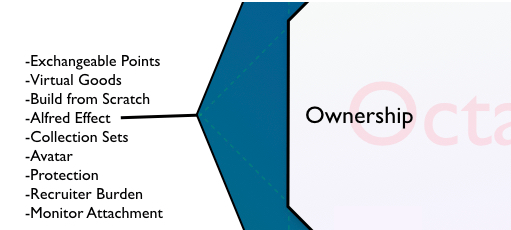
\includegraphics[width= 0.3\textwidth]{images/core-drive-4-ownership-and-possession.png}
    \end{center}
This is the drive where users are motivated because they feel like they own something. When a player feels ownership, she innately wants to make what she owns better and own even more. Besides being the major core drive for wanting to accumulate wealth, this deals with many virtual goods or virtual currencies within systems. Also, if a person spends a lot of time to customize her profile or her avatar, she automatically feels more ownership towards it too. Finally, this is also the core drive that makes collecting stamps or puzzle pieces fun.

      \item \textbf{Core Drive 5: Social Influence \& Relatedness}
    \begin{center}
        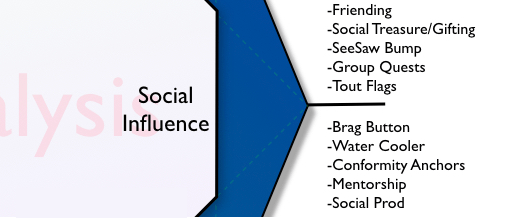
\includegraphics[width= 0.3\textwidth]{images/core-drive-5-social-influence-and-relatedness.png}
    \end{center}
This drive incorporates all the social elements that drive people, including: mentorship, acceptance, social responses, companionship, as well as competition and envy. When you see a friend that is amazing at some skill or owns something extraordinary, you become driven to reach the same level. Also, it includes the drive we have to draw closer to people, places, or events that we can relate to. If you see a product that reminds you of your childhood, the sense of nostalgia would likely increase the odds of you buying the product. This Core Drive is relatively well-studied too, as many companies these days are putting a lot of priority on optimizing their online social strategies.

      \item \textbf{Core Drive 6: Scarcity \& Impatience}
    \begin{center}
        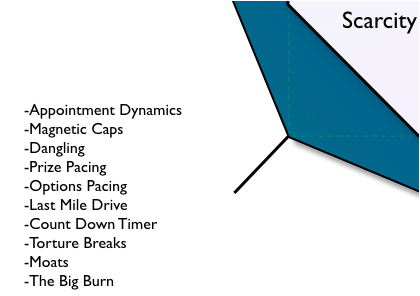
\includegraphics[width= 0.3\textwidth]{images/core-drive-6-scarcity-and-impatience.png}
    \end{center}
This is the drive of wanting something because you can’t have it. Many games have Appointment Dynamics (come back 2 hours later to get your reward) – the fact that people can’t get something right now motivates them to think about it all day long. This is the Core Drive utilized by Facebook when it first started: at first it was just for Harvard. Then it opened up to a few other prestigious schools, and eventually all colleges. When it finally opened up to everyone, many people wanted to join because they previously couldn’t get in it.

      \item \textbf{Core Drive 7: Unpredictability \& Curiosity}
    \begin{center}
        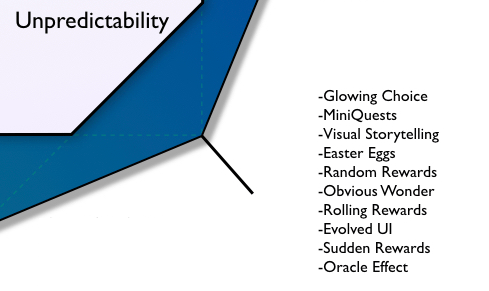
\includegraphics[width= 0.3\textwidth]{images/core-drive-7-unpredictability-and-curiosity.png}
    \end{center}
Generally, this is a harmless drive of wanting to find out what will happen next. If you don’t know what’s going to happen, your brain is engaged and you think about it often. Many people watch movies or read novels because of this drive. However, this drive is also the primary factor behind gambling addiction. Also, this core drive is utilized whenever a company runs a sweepstake or lottery program to engage users. The very controversial Skinner Box experiments, where an animal irrationally presses a lever frequently because of unpredictable results, are exclusively referring to the core drive of Unpredictability \& Curiosity, although many have misunderstood it as the driver behind points, badges, and leaderboard mechanics in general.

      \item \textbf{Core Drive 8: Loss \& Avoidance}
    \begin{center}
        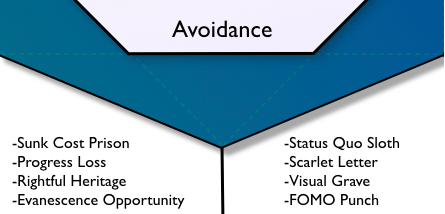
\includegraphics[width= 0.3\textwidth]{images/core-drive-8-loss-and-avoidance.png}
    \end{center}
This core drive is based upon the avoidance of something negative happening. On a small scale, it could be to avoid losing previous work. On a larger scale, it could be to avoid admitting that everything you did up to this point was useless because you are now quitting. Also, opportunities that are fading away have a strong utilization of this Core Drive, because people feel like if they didn’t act immediately, they would lose the opportunity to act forever.
\end{itemize}

\subsection{Left Brain vs. Right Brain}
\begin{center}
    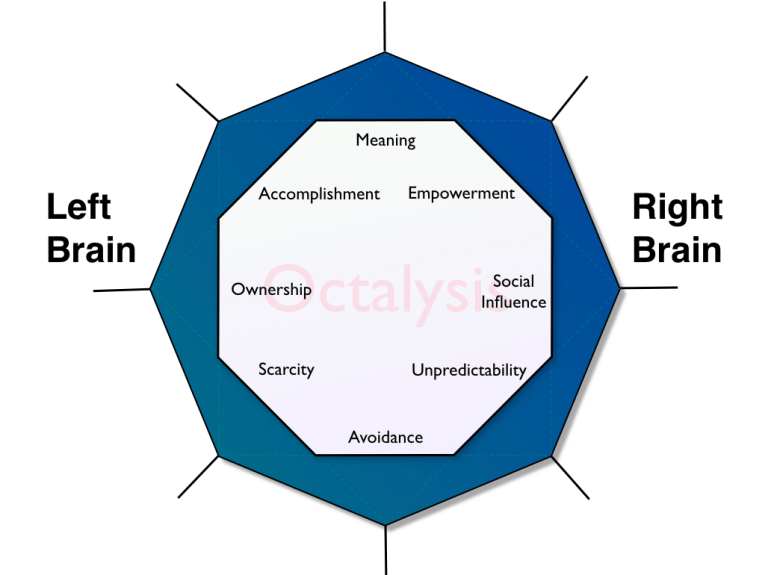
\includegraphics[width=0.6\textwidth]{images/left-brain-vs-right-brain-core-drives.png}
\end{center}
\begin{itemize}
    \item ''The Octalysis Framework is arranged so that the Core Drives that focus on creativity, self-expression, and social dynamics are organized on the right side of the octagon. In my framework I call them Right Brain Core Drives. The Core Drives that are most commonly associated with logic, analytical thought, and ownership are graphed on the left side of the octagon and are termed Left Brain Core Drives.''
\item ''Left Brain Core Drives tend to rely on Extrinsic motivation - you are motivated because you want to obtain something[..]. On the other hand, Right Brain Core Drives are mostly associated with Intrinsic Motivations - you don't need a goal or reward to use your creativity, hangout with friends, or feel the suspense of unpredictability - the activity itself is rewarding on its own.''
\item '' [M]any companies emphazise designing for Extrinsic Motivatiors, such as providing a reward when they complete a task. However, many studies have shown that extrinsic motivation impairs intrinsic motivation. Why? Because once the companies stop offering the extrinsic motivator, user motivation will often plummet to a level much lower than when the xtrinsic motivator was first introduced.''
\end{itemize}


\subsection{White Hat vs. Black Hat Gamification}
\begin{center}
    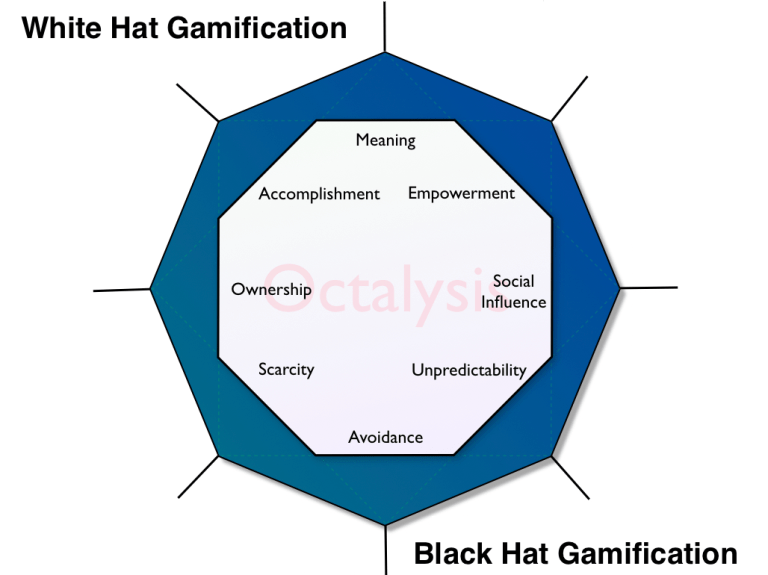
\includegraphics[width=0.6\textwidth]{images/white-hat-vs-black-hat-gamification.png}
\end{center}
''Another element to note within Octalysis is that the top Core Drives in the octagon are considered very positive motivators, while the bottom Core Drives are considered negative motivators.\\
\\
Techniques that utilize the top Core Drives are called “White Hat Gamification”,while techniques that utilize the bottom Core Drives are called “Black Hat Gamification”.\\
\\
If something is engaging because it lets you express your creativity, makes you feel successful through skill mastery, and gives you a higher sense of meaning, it makes users feel very good and powerful.\\
\\
On the other hand, if you are always doing something because you don’t know what will happen next, you are constantly in fear of losing something, or because there are things you can’t have, even though you would still be extremely motivated to take the actions, it can often leave a bad taste in your mouth.\\
\\
The problem with Zynga games [see \url{https://de.wikipedia.org/wiki/Zynga} for more information], according to the Octalysis framework, is that they have figured out how to do many Black Hat Game Techniques, which drive up revenue numbers from users, but it doesn’t make users feel good. So when a user is finally able to leave the system, they will want to, because they don’t feel like they are in control over themselves, just like gambling addiction.\\
\\
Keep in mind that just because something is Black Hat doesn’t mean it is necessarily bad – these are just motivators – and they can be used for productive and healthy results or malice and manipulative ones. Many people voluntarily submit themselves into Black Hat Gamification in order to go to the gym more often, eat healthy, or avoid hitting the snooze button every morning.\\
\\
A good Gamification expert will consider all 8 Core Drives on a positive and productive activity so that everyone ends up happier and healthier.'' (from his block)\\
\\
You are able to create an octagon for your personal application at \url{https://yukaichou.com/octalysis-tool/}

\subsection{Level 2 Octalysis Design for All 4 Phases}
\begin{itemize}
    \item There are more than 5 levels of the Octalysis design.
    \item ''Level 2 Octalysis, where we try to optimize experiences throughout all 4 phases of the player/user journey:
    \begin{enumerate}
        \item Discovery (why people would even want to try out the experience)
        \item Onboarding (where users learn the rules and tools to play the game)
        \item Scaffolding (the regular journey of repeated actions towards a goal)
        \item Endgame (how do you retrain your veterans)
    \end{enumerate}
    \item Most people treat their product as one experience, which seems reasonable. But in terms of motivation, I believe this is a mistake because the reason you are using a product on Day 1 is often very different from that of Day 100. Since everything you do is because of one of these Core Drives. If at any phase none of [them] is presented there is no reason for the user to move to the next phase.
    \item In the following ''illustration, you can evaluate how different Core Drives are more prominent during each Experience Phase[..].
    \begin{center}
            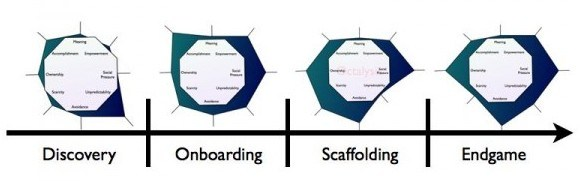
\includegraphics[width=0.6\textwidth]{images/Gamification-Octalysis.018-e1363796378415.jpg}
    \end{center}
\end{itemize}

\subsection{Level 3: Player Types}
\begin{center}
    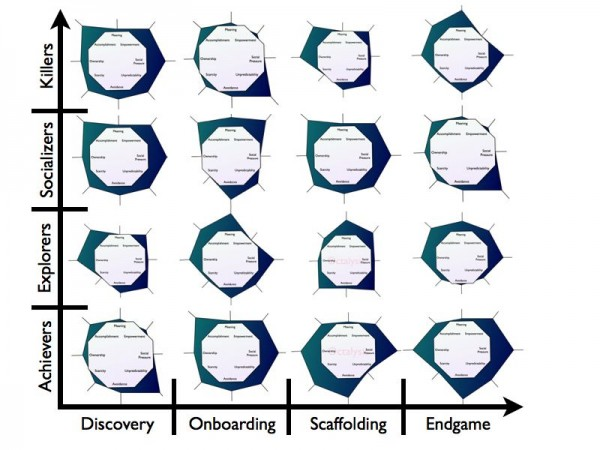
\includegraphics[width=0.5\textwidth]{images/Gamification-Octalysis.020.jpg}
\end{center}
\begin{itemize}
    \item In this diagram, Richard Bartle's Four Player Types are applied which is the most recognized model in game design.
    \item Bartle claims ''that is Four Player Types may not be suitable for gamification environments''.
    \item The point here is that different types of people are motivated differently, so Level 3 Octalysis allows the designer to understand and design for how everyone is feeling at different stages.''
    \item While there are five levels of Octalysis in total, Level 1 is often sufficient for the majority of companies seeking to understand why their products are not engaging their users. Higher-level Octalysis processes are useful for organizations that are truly commited to making sure that they push their metrics in the right direction and improve longevity of a gamified system.'' 
\end{itemize}

\newpage

\section{Chapter 4: Putting Gamification in its Place}
\subsection{Explicit Gamification: Games that Fulfill Non-Game Purposes}
\begin{itemize}
    \item ''The two types of gamification implementations in my own work are ''Implicit Gamification'' and ''Explicit Gamification''.
    \item ''Explicit Gamification involves strategies that utilize applications that are obviously game-like. Users acknowledge they are playing a game, and generally need to pot into playing.''
    \item Examples for Explicit gamification: 
    \begin{itemize}
        \item Dikembe Mutombo's 4 1/2 weeks to Save the World
        \item McDonald's Monopoly Game
        \item FoldIt
        \item Undiscovered Territory
        \item Repair the Rockaways
    \end{itemize}
    \item ''The advantage of designing for explicit gamification is that the product is generally more playful and it allows the designer to have more freedom of creativity. The disadvantage is that it could be seen as childish, non-serious, or distracting to some target users such as enterprise firms, banks or manufacturers.''
\end{itemize}

\subsection{Implicit Gamification: Human-Focused Design that Utilizes Game Elements}
\begin{itemize}
    \item ''Implicit Gamification is a form of design that subtly employs gamification techniques and the 8 Core Drives of Octalysis into the user experience. Implicit Gamification techniques are filled with game design elements that are sometimes even invisible to the user.''
    \item Examples:
    \begin{itemize}
        \item LinkedIn Progress Bar
        \item intrinsic motivation that drives Wikipedia
        \item competitive bidding system and feedback system via eBay
        \item social comparison and motivation in OPower
        \item Unpredictability and scarcity within Woot!
    \end{itemize}
    \item '' The advantage of implicit gamification is that it is technically easier to implement and can be approriate in most contexts. The disadvantage [...] is that this very convenient implementation can often lead to ''lazy'' design where the subtle game dynamics are incorrectly designed for and sloppily put together. This would lead to something completely ill-formed or ineffective in terms of driving business metrics.''
\end{itemize}

\subsection{Implicit vs. Explicit Gamification}
\begin{itemize}
    \item ''One type of gamification is not inherently better than the other.''
    \item ''The proper use of Implicit or Explicit Gamification depends on the purpose of the project as well as your target market.''
    \item ''All 8 Core Drives can be implemented into Implicit and Explicit Gamification campaigns.''
\end{itemize}

\newpage

\section{Chapter 5: The First Core Drive - Epic Meaning \& Calling}
\begin{itemize}
    \item ''When it comes to Epic Meaning \& Calling, it's not about what you want as an individual nor about what makes you feel good. Individuals participate in the system and take action not because it necessarily benefits them, but because they can see themselves as heros of a grander story. It's about playing your part for the greater good.''
    \item Core Drive 1 ''is generally best communicated during the Discovery and Onboarding Phase of a Player's Journey. You want to communicate very eraly on exactly why the user should participate in your mission and become a player.''
    \item Examples:
    \begin{itemize}
        \item Apple selling a vision
        \item Waze using a metaphor for traffic - picturing it as a monster and asking people to help them defeating it
    \end{itemize}
    \item ''The powerful thing about Epic Meaning \& Calling is that it turns otherwise passive users into powerful evangelists of your mission. They are even highly forgiving of your flaws.''
    \item important factor for Core Drive 1: ''It must feel authentic''
\end{itemize}

\subsection{Game Techniques within Epic Meaning \& Calling}
    \subsubsection{Narrative (Game Technique \#10)}
        \begin{itemize}
            \item ''One of the [...] effective ways to instill Epic Meaning \& Calling into your user base is trough an engaging Narrative. This allows you to introduce a story that gives people context for a higher meaning trough interacting with your company, product or web-site.''
            \item Example: Zamzee, a ''wearable technology''
        \end{itemize}
        
    \subsubsection{Humanity Hero (Game Technique \#27)}
    \begin{itemize}
        \item ''If you can incorporate a world mission into your offerings, you can gain even more buy-in during the Onboarding process.''
        \item Examples:
        \begin{itemize}
            \item TOM's Shoes: Sends one pair of shoes to a child in a third-world country whenever you place an order with them.
            \item FreeRice.com: Donates 10 grains of rice for every correct answer to the educational questions posted on their site.''
        \end{itemize}
    \end{itemize}
    
    \subsubsection{Elitism (Game Technique \#26}
    \begin{itemize}
        \item ''Allowing your users [...] to form a prideful group based on ethnicity, beliefs, or common interets also makes them feel like they are part of a larger cause. Elitism instills group pride, which means each member tries to secure the pride of the group by taking specific actions. The group also attempts to frustrate rivals, which can lead both groups upping their actions to beat the competition.''
        \item Examples
        \begin{itemize}
            \item Rivalry between schools/universities/sport clubs
            \item Kiva.org: Comparison between Christians and Atheists - who donates more?
        \end{itemize}
    \end{itemize}
    
    \subsubsection{Beginer's Luck (Game Technique \#23)}
    \begin{itemize}
        \item ''Begginer's Luck focuses part [...]. Calling makes people think they are uniquely destined to do something. With Begginer's Luck, people feel like they are one of the few chosen to take action - which makes them much more likely to take it.''
    \end{itemize}
    
    \subsubsection{Free Lunch (Game Technique \#24)}
    \begin{itemize}
        \item ''Giving freebies (that are normally not free) to select people in such a way that it binds them to a larger theme can make customers feel special and encourage them to take further action'.'
    \end{itemize}
    
    \subsection{Believability is Key}
    Even though Epic Meaning \& Calling is powerful [..], it can also backfire and fail in epic proportions. As you use these concepts, keep in mind, that you can really turn people off when you're appearing disingenuous in your efforts to create Epic Meaning and Calling.''
    
    \subsection{Core Drive 1: The Bigger Picture}
    \begin{itemize}
        \item ''It underlines the purpose behind the activity and strengthens all the other seven Core Drives when it is introduced correctly.''
        \item Its ''weakness lies in the difficulty of implementing believability, as well as the lack of urgency within the motivation. While people constantly aspire tobecome part of something bigger and would feel great if they actually took the actions, they will often procrastinate and delay those very actions. Thus, to create desirable behaviour, the gamification designer needs the help of the other Core Drives[...].''
        \item TEDx talk on how eight different world-changing products utilize each of the 8 Core Drives can be accessed at \url{https://www.youtube.com/watch?v=v5Qjuegtiyc}
    \end{itemize}

\newpage

\section{Chapter 6: The Second Core Drive - Development \& Accomplishment}
\begin{itemize}
    \item ''This is the Core Drive where people are driven by a sense of growth and a need to acomplish a targeted goal. It is what focuses us on a career path, generates our enthusiasm and commitment to learning a new skill, and ultimately motivates us by showing us how far we've come and how much we've grown.''
    \item ''This is also the most common implementation of gamification we see in the market, as most of the PBLs - points, badges, and leaderboards - appera heavily in this drive.
\end{itemize}

\subsection{Development \& Accomplishment in Games}
\begin{itemize}
    \item ''Almost all games show you some type of progress towards the Win-States. A Win-State is often a scenario where the user has overcome some sort of challenge [...]. Games break down user challenges into stages to help the user feel like there is always progress.''
    \item ''Our brains have a natural desire to achieve goals and to experience growth in order to feel that real progress in life is being made.''
    \item The key to Core Drive 2 [...] is to make sure users are proud of overcoming the challenges that are set out for them. Jane McGonigal, renowned game designer and Ph.D. in Performance Studies, defines games as ''unnecessary obstacles that we volunteer to tackle.'''' (book from her ''Reality is broken'' penguin book grop ny, 2011)
    \item ''McGonigal points out that challenges and limitations are what makes a game fun.''
\end{itemize}

\subsection{The First Gamification Site that I was Addicted to}
\begin{itemize}
    \item ebay's design elements:
    \begin{itemize}
        \item Rewarding system for sellers according to the amount of items they sold over ebay and how many positive ratings they get.
        \item There is a game element ''Torture Break'' (''a user must wait an interval of time regardless of their actions, a game technique to be explored under Core Drive 6'') when no one bits on your item for a long time.
        \item suspense is created by the biding system - creates a sense of urge.
        \item Sellers get certificates according to their engagement (sold item and good ratings).
        \item Buyers feel like they have won when retrieving an item because they had to go against other people. They are even paying more than the item is worth sometimes.
        \item Quickly outbiding each other before the time runs out contains 2 game techniques. ''The effect is a combination of a Coundown Timer and a Last Mile Drive, where users feel that they are so close to the goal that they rush to complete it. [...] These mostly employ Black Hat techniques.''
    \end{itemize}
\end{itemize}

\subsection{Never make Users Feel Dumb}
\begin{itemize}
    \item ''Beyond improving one's ranks and obtaining badges, a very important type of emotional accomplishment is to ''feel smart''.''
\end{itemize}

\subsection{Star of Bethlehem - Guiding Users Forward}
\begin{itemize}
    \item ''Feeling a sense of progress and ultimately losing is much better than feeling stuck and confused. If you playthe game through and lose, your natural reflection is to start a new game; but if you get stuck [..] for a long period of time, you may just abandon the game altogether and start doing other things.''
    \item To prevent this from happening you could use the game technique ''Glowing choice, where a user is visually guided by obvious signs towards how to proceed.''
    \item This shown possibility of process does not have to be the best choice and could even lead to failure when chosen (repeatedly). E.g. Candy Crush help.
    \item You can also mark directions or choices you want the user to make.
    \item ''It is important to note that this Desired Action is'' marked in a special way. For this we use the game technique Desert Oasis, ''where visually nothing else is prominent besides the main Desired Action.''
    \item Example for this is an item page of Amazon. Only the Buy option are marked colorful or when looking at a book there often is a big orange arrow to invent people into looking into the book.
\end{itemize}

\subsection{Game Techniques within Development \& Accomplishment}
\subsubsection{Progress Bars (Game Technique \#4)}
\begin{itemize}
    \item ''Our brains hate it when incomplete things are dangled in front of our faces.''
\end{itemize}

\subsubsection{The Rockstar Effect (Game Technique \#92)}
\begin{itemize}
    \item ''The Rockstar Effect is a gamification design technique where you make users feel everyone is dying to interact with them. In essence, if you make people feel like they have raned their way in becoming a Rockstar, they will feel so much pride in that they will continue to perform the Desired Actions of building up an even greater fanbase and sharing with others.''
    \item Example: Twitter's one-way follow.\\
    ''Many people saw getting many followers as a true achievement - meaning that everyone wanted to listen to your valuable opinions'' while you could ''ignore'' them.
    \item ''At one point, influential people started to compete with eachh other to see who had more followers.''
\end{itemize}

\subsubsection{Achievement Symbols (Game Technique \#2)}
\begin{itemize}
    \item ''Bages are what I call ''Achievement symbols'' and can come in many forms - badges, stars, belts, hats, uniforms, trophies, medals, etc.. The important thing about Achievement Symbols is that they must symbolize ''achievement''.''
    \item ''If trough your creative skills you solved a unique problem that not everyone could solve, and as a result received a badge to symbolize that achievement, you feel proud and accomplished.''
    \item ''Achievement symbols merely reflect achievement, but are not achievement by themselves.''
\end{itemize}

\subsubsection{Status Points (Game Technique \#1)}
\begin{itemize}
    \item ''There are two types of points in a motivation system: Status Points and Exchangeable Points. Status Points are for keeping score of progress. Internally, it allows the system to know how close players are towards the win-state. Externally, it gives players a feedback system for tracking their progress.''
    \item ''Showing people their score and how it changes based on small improvements often motivates them towards the right directions.''
    \item ''Within Status Points, there are also smaller divisions of types. For example, Absolute Status Points (which measure the total amount of points earned during a journey) versus Marginal Status Points (which are points that are specifically set for a given challenge or one time period, and can be reset once that challenge or time period is over).''
    \item ''One-Way Status Points (points that can only go up) versus Two-Way Status Points (it can also go down as the user fails to achieve the Win-State).''
    \item ''How you craft the gain and loss of points, as well as meaning behind the points can significantly change the users' perception of your product.''
    \item ''With the rules you set, you are establishing an interaction with the user and communicating your values.''
    \item ''If you give people a bunch of points just to do marketing for you, or reward them with virtual items for every little stupid thing, users will feel like the game is shallow.''
    \item ''Users have no interest in a game if they know the game designer is just trying to benefit themselves instead of caring about their community.''
    \item ''When you design your Status Point system, make sure it is based om something meaningful - something that the users themselves want to stress people out.''
\end{itemize}

\subsubsection{Leaderboards (Game Technique \#3)}
\begin{itemize}
    \item ''Leaderboards is a game element where you rank users based on a set of criteria that is influenced by the users' behaviour towards the Desired Action.''
    \item ''If you use a site for a few hours and receive 25 points, and then see the Top 20 list that number 20 already has 25,000,000 points, that would likely discourage you from trying further.''
    \item ''What users need is Urgent Optimism, another term coined by Jane McGonigal, where the user feels optimistic that they can accomplish the task, but also the urgency to act immediately.''
    \item ''There are a couple of variations that have shown to perform more effectively:
    \begin{itemize}
        \item ''First, you always want to position the user in the middle of the leaderboard display, so all they see is the player ranked right above them and the player ranked just below. It's not very motivating in seeing how high the Top 10 players are, but it's incredibly motivating when one sees someone who used to be below them suddenly excelling.''
        \item Another variation that has proved successful is to set up Group Leaderboards where the ranking is based on the combined efforts of a team. In this case, even though not everyone is competitive and needs to be at the top, most people don't want to be laggard that drags the team down. As a result everyone works harder because of Social Influence \&Relatedness (Core Drive 5).''
        \item ''The next variation is to set up constantly refreshing leaderboards, where every week the data would refresh and the leaderboards will start tracking progess anew.''
        \item Finally, it's a good idea to implement micro-leaderboards, where only the users' friends or very similar people are compared.''
    \end{itemize}
    \item ''The key way to effectively integrate a leaderboard is to ensure that the user can quickly recognize the action items that drives them to reach win-state. If there is no way of achievement, there is no action.''
\end{itemize}

\subsection{Core Drive 2: The Bigger Picture}
\begin{itemize}
    \item ''Since Development \& Accomplishment is the easiest Core Drive to design for, many companies focus on this Core Drive sometimes almost exclusively.''
    \item '' Is often a natural result after good implementation of other Core Drives, such as Core Drive 3: Empowerment of Creativity \& Feedback, Core Drive 4: Ownership \& Possession, as well as Core Drive 6: Scarcity \& Impatience.''
    \item ''Often, it also leads to Core Drive 5: Social Influence \& Relatedness, where the user wants to share with their friends that sense of achievement and accomplishment.''
\end{itemize}

\newpage

\section{Chapter 7: The Third Core Drive - Empowerment of Creativity \& Feedback}
\begin{itemize}
    \item ''Can remove the so-called ''gamification-fatigue.'''' (Becoming tired of a game and eventually abandon it)
    \item ''Hopefully the system that you are designing actually has a purpose to it, and so even if it becomes boring (which is probably the current state anyway), your users still have a reason to stay on.''
    \item ''When a user can continuously tap into their creativity and derive an almost limitless number of possibilities, the game designer no longer needs to constantly create new content to make things engaging''
    \item Examples: Starcraft, Poker, Golf, Chess, Mahjong
\end{itemize}

\subsection{Tic-Tac-Draw}
\begin{itemize}
    \item ''When you design a great gamified system, you want to make sure there isn't one standard way to win. Instead, provide users with enough meaningful choices that they can utilize drastically different ways to better express their creativity, while still achieving the Win-State''
\end{itemize}

\subsection{The General's Carrot in Education}
\begin{itemize}
    \item ''When you design for Core Drive 3: Empowerment of Creativity \& Feedback, it is important to create a setup where the user is given a goal, as well as a variety of tools and methodologies to strategize towards reaching that goal. Often your users are not motivated because they don't understand the purpose of the activity, do not clearly identify the goal of the activity, and/or lack meaningful tools to create expressive strategies to reach the goal.''
\end{itemize}

\subsection{The Downfall of Draw Something}
\begin{itemize}
    \item Many users typically start to drop out when a game fails ''to provide fresh content and challenges that would give people a sense of continued improvement and novel conditions for further mastery.''
    \item E.g. when words repeat to often in Draw Something ''(essentially Pictionary, where one side draws something with a pen and the other side guesses)''
\end{itemize}

\subsection{Game Techniques within Empowerment of Creativity \& Feedback}

\subsubsection{Boosters (Game Technique \#31)}
    \begin{itemize}
        \item Boosters = '' a player obtains something to help them achieve the win-state effectively.''
        \item Example: mushroom or flower from Super Mario
        \item They are usually limited to certain conditions. e.g. limited time or loosing the booster when being injured
        \item They can be earned or bought
        \item The ''feeling of being empowered with new, but limited power-ups is exhilarating and an extremely strong motivator towards the desired action.''
    \end{itemize}
    
\subsubsection{Milestone Unlock (Game Technique \#19)}
\begin{itemize}
    \item ''One of the most successful design techniques within games is something that I call the Milestone Unlock. When people play games, they often set an internal stop time in the form of a milestone - ''Let me beat this boss and then I'm done.'''' e.g.
    \item ''What the Milestone Unlock does is open up an exciting possibility that wasn't there before that milestone was reached.''
    \item ''Once players level up (their ''stop-time-milestone''), they naturally want to see what these new skills are like. They will want to test them out a bit, then test them out on stronger enemies, enjoy how powerful they are, and then realize they are so close to the next milestone that they might as well get there before stopping. This is when people plan to stop at 11PM but end up playing till 4AM.
\end{itemize}

\subsubsection{Poison Picker/Choice Perception (Game Technique \#89)}
    \begin{itemize}
        \item ''Many studies have shown that people like something more when they are given a choice, compared to simply having one option. This holds true even if the multiple options are not as appealing compared to the single choice.''
        \item E.g. Your parents tell you that you have to play an instrument but you can chose which one you would like.
        \item ''The key to the Choice Perception is that the choice itself is not necessarily meaningful, but merely makes a person feel like they are empowered to choose between different paths and options.'' (E.g. you are still forced to play an instrument)
        \item ''When I say the choice is not meaningful, it could mean that either the user is presented with a good option and a bad option, inviting the user to naturally choose the better one [...]; or it could mean that all the options are too limiting and therefore undifferentiated from one another.''
        \item ''Jesse Schell, in his book \textit{The Art of Game Design - A Book of Lenses}, introduces two Lenses: The Lens of Freedom and the Lens of Indirect Control. Schell describes that, ''\textit{we don't always have to give the player true freedom. [...] if a clever designer can make a player feel free, when really the player has very few choices, or even no choice at all, then suddenly we have the best of both worlds - the player has the wonderful feeling of freedom, and the designer has managed to economically create an experience with an ideal interest curve and an ideal set of events.}''''
        \item ''According to Schell, this can be accomplished by 1) Adding constrains to player choices, 2) Incentivizing players to take certain choices that actually meets the players goals, 3) Create an Interface that guides the user towards the Desired Actions, 4) Adding visual designs to attract the player's sight, 5) Provide social guidance (often trough computer generated characters in the game), and 6) Music control that affects player behaviours.''
        \item ''Choice Perception influences our decisions in many other significant ways, such as wasting time and energy keeping meaningless doors or options open, even though they were formerly written off as bad options, simply to maintain a perception of having a choice.''
        \item ''Since Choice Perception suggests a lack of meaningful choices, it often is not ideal in an implementation as it does not truly bring out the creativity of the user. You could also offend users if too many options are blatantly meaningless.''
     \end{itemize}
     
\subsubsection{Plant Picker/Meaningful Choices (Game Technique \#11)}
\begin{itemize}
    \item ''Beyond choices that allow people to feel like they are empowered, there are choices that are truly meaningful and demonstrates preferences that are not obviously superior over others. I refer to these techniques as ''Plant Pickers'' because, just like deciding what to plant in a garden, it is often a preference on style and strategy, something that fuels Core Drive 3.''
    \item ''If you create a gamified environment with a hundred players, and all hundred of these players reach the Win-State in the exact same way (such as ''do action A, get points, do action B, get badges, do action C, win!''), there are no meaningful choices present.''
    \item ''If all hundred players play the game differently, then you have a great amount of meaningful choices.''
    \item That level of meaningful choices and play is the ultimate state of Core Drive 3: Empowerment of Creativity \& Feedback.''
    \item ''If thirty players play the game one way, thirty players another way, and the last fourty players yet another way, then you have some level of Meaningful Choices.''
    \item Examples: Plants vs. Zombies, Farmville (Art)
\end{itemize}

\subsection{Core Drive 3: The Bigger Picture}
\begin{itemize}
    \item It ''is a great Core Drive on many different levels. It taps into our innate desire to create, by providing us the tools and power to direct our own gameplay and giving us the ability to affect the environment around us trough our imagination.''
    \item Often the most difficult Core Drive to implement
\end{itemize}

\newpage

\section{Chapter 8: The Fourth Core Drive - Ownership \& Possession}
\begin{itemize}
    \item ''It represents the motivation that is driven by our feelings of owning something, and consequently the desire to improve, protect, and obtain more of it.''
    \item ''Core Drive 4 is connected to our investment of time or resources into customizing something to our own liking.''
    \item ''Here decisions are mostly based on logic and analysis, reinforced by the desire for possession as the primary motivating factor.''
    \item Example: Farmville
\end{itemize}

\subsection{Wait, it's mine? Hold on, I do care then!}
\begin{itemize}
    \item ''Once you feel a sense of ownership over something, its status elevates and it begins to motivate your behavior differently.''
\end{itemize}

\subsection{Stamps of Sanity}
\begin{itemize}
    \item ''One of the most common manifestations of the Ownership \& Possession Core Drive is the desire to collect things, such as stamps or baseball cards.''
    \item ''they are only meaningful because they represent a piece in a larger set.''
    \item ''Some readers might feel that Core Drive 4 only entails the actions of accumulating more possessions, but it also provides emotional comfort to those who simply dwell upon those possessions.''
    \item ''It not only has the ability to engage, it has the ability to comfort and instill a sense of well-being. You see this phenomenon with baseball cards, pens [...]. People just like to display them and marvel at the collection for hours, while seemingly ''having fun'' in the process.''
\end{itemize}

\subsection{The Perfect Pet}
\begin{itemize}
    \item ''When people feel like they have ownership of something, they naturally want to care for it and protect it.''
    \item Example: Pet Rock
\end{itemize}

\subsection{The First Virtual Pet}
\begin{itemize}
    \item The ''ingrained sense of Ownership \& Possession, along with some added benefits of novelty (Core Drive 7: Unpredictability \& Curiosity), made products like Pet Rocks, Tamagotchi, and later on Facebook games like Farmville or Pet Society such big successes worldwide.
\end{itemize}

\subsection{The Endowment Effect}
\begin{itemize}
    \item ''When a person starts to own something, they immediatly place more value on that item relative to others who don't own it.''
    \item Examples:
    \begin{enumerate}
        \item A ''well-respected academic and wine lover becomes very reluctant to sell a bottle of wine from his collection for 100\$, but would also not pay more than 35\$ for a wine of similar quality.''
        \item Research were students had to go through a demanding process of obtaining tickets for a basketball game. They had to camp outside and pay attention to specific signals for a hole semester only to be ''lucky'' to retrieve a lottery ticket. Then the lottery was performed, deciding the winners of the tickets. Afterwards people who didn't get a ticket were asked how much they would pay for a ticket. On average they were willing to pay 170\$. On the other hand, people who won a ticket were asked for how much they would sell it. They were demanding 2,400 \$ on average, even though they had gone through the same troubles as the other to gain a lottery ticket.
    \end{enumerate}
    \item ''The Endowment Effect is also realized when we simply imagine ourselves owning something.'' It was found out that ''within auction sites, the longer people remained the top bidder (having imagined themselves as the official owner for longer), the more aggressively they would bid when someone offered a counter bid. The envisioned ownership actually motivates people to fight for their divine rights to that item they don't yet own.''
\end{itemize}

\subsection{For Sale Not For Use}
\begin{itemize}
    \item ''One caveat to the Endowment Effect is, if the person owns something as a token ''for exchange'', they will not feel attached to the item in a biased matter.''
    \item Example: ''If a merchant owns hundreds of shoes in the hopes of exchanging them for money, he obviously does not feel that sense of attachment when someone buys the product.''
\end{itemize}

\subsection{Identity, Consistency, and Commitments}
\begin{itemize}
    \item ''Another interesting effect of Core Drive 4 [...] is that it also drives us to value our own identity and become more consistent towards our past.''
    \item ''In fact, science has shown that the longer we live, the more attached we become to our existing beliefs, preferences, methodologies, and even our own names.''
    \item ''A [...] study [...] revealed that people are much more likely to choose careers that sound similar to their own names.''
    \item ''Moreover people tend to move to places that are similar to their own names too.''
\end{itemize}

\subsubsection{Consistency}
\begin{itemize}
    \item ''Stemming from the attachment to our own identities is the need to behave consistently with our past actions. Dan Ariely describes this as seslf-herding, where we believe something is good (or bad) on the basis of our previous behaviour.''
    \item Examples: 
    \begin{itemize}
        \item ''Often we buy certain items and brands just because we bought them in the past and we would like to stay consistent with our own choices, even though the product or brand may no longer be the best for our current needs.''
        \item Being more likely to believe that a horse is going to win a race just because we bed on it
    \end{itemize}
    \item ''Our need to be consistent with our past can also cause us to do unreasonable things for others.''
\end{itemize}

\subsubsection{Commitments: The Power of Writing Something Down}
\begin{itemize}
    \item ''Our need of consistency becomes even stronger when we create a commitment, especially when we write it down.''
    \item Example: Study were students had to estimate the length of lines. There were three groups. The first just had to think the estimation in their head. The second group had to write it down but without anyone else knowing their estimation and the third group had to write it down and tell the other participants their guess. Afterwards the researchers gave new misleading information that suggested the students' initial estimates were incorrect and gave them a chance to change their answers. The group that just had to think their estimation were the most likely ones to change their result. Those who had to write it down were not so likely to change their estimation and the group that had to write it down and say it out loud was even unlikelier to change their opinion.
\end{itemize}

\subsection{Game Techniques within Ownership \& Possession}

\subsubsection{Build-From-Scratch (Game Technique \#43)}
    \begin{itemize}
        \item ''When you create a product or service, it is often desirable for your users to increase their vested ownership in the process of its creation. This is why it is useful to have them involved in the development process early on [...].''
        \item ''Building something from scratch means that instead of giving them the entire setup - giving them the the fully furnished house [...], you want them to start off decorating the house from scratch.''
        \item ''When people are building something from scratch, they feel like, ''I own this. This is my thing.''
        \item ''If the Build-From-Scratch technique distracts people away from the first Major Win-State (where users first exclaim, ''Wow! This is awesome!''), then it is not a good design. Either you should give users the option to Build-From-Scratch with some quick template options that will allow them to move forward  quickly and customize later, or you want to ensure that the Build-From-Scratch Technique itself is a First Major Win-State that users feel exited about.''
    \end{itemize}   
    
\subsubsection{Collection Setts (Game Technique \#16)}
    \begin{itemize}
        \item ''One  of the most powerful and effective ways to utilize Core Drive 4''
        \item ''Say you give people a few items, characters or badges, and you tell them that this is part of a collection set that follows a certain theme. This creates a desire in them to collect all the elements and complete the set.''
        \item ''When you give users rewards, don't just give them physical items directly, for those generally have less motivational longevity. More often, giving them collection pieces will result in longer-term engagement.''
        \item ''When a user expects a full reward either due to your own advertising or because of what your competitors are advertising, giving them a Collection Set piece can sometimes backfire and end up insulting that user.''
        \item Example: Geomon, Pokémon, McDonald's Monopoly Game
    \end{itemize}
    
\subsubsection{Exchangeable Points (Game Technique \#75)}
    \begin{itemize}
        \item ''Users can utilize their accumulated points in a strategic and scarce manner to obtain other valuables. Exchangeable Points can have various types of uses. There are no points that can only be redeemed within the game economy for valuables, or points that can be traded with other players in the same system. Some exchangeable points allow users to trade with people outside of the gamified system where they were originally earned in. Each of these types of points has pros and cons, and many good gamified systems [...] have a combination of the above to ensure their economy maintains its value for its users.''
        \item ''It is difficult to run an effective economy. You have to carefully consider the correct labor-to-time-to-tradability-to-reward ratios while constantly adjusting the balance to ensure that people continue valuing your points and currency system. If the system no longer rewards the appropriate labor with the commensurate perceived value, then the economy loses its legacy.''
        \item ''One of the key points to pay close attention to is the scarcity control of the economy. This means that users should never feel like the exchangeable currency or goods are excessively abundant. This is often controlled by the true scarcity of time where labor in the system is balances against the resulting rewards.''
    \end{itemize}
    
\subsubsection{Monitor Attachment (Game Technique \#42)}
    \begin{itemize}
        \item ''Monitor Attachment is a game technique that allows people to develop more ownership towards something, such that they are constantly monitoring or paying attention to it.''
        \item ''When users are monitoring the state of something, they naturally want that state to continually improve. If you are constantly looking at the progression of some numbers, you automatically grow more engaged with the success and growth of these numbers.''
        \item E.g. it can ''be identified in the relationship developed over time with a favorite local coffee shop'' (amongst other things). $\Rightarrow$ ''You build familiarity with the shop, which in turn makes you feel like you partially ''own'' the place as a committed community member and customer.''
        \item 'This is the ''tendency of liking something we feel familiar with''.
        \item ''Because our subconscious minds are bad at differentiating between things that are safe, comfortable, desirable, our brain automatically associates it with something that is safe and desirable. Cognitive ease plays a substantial part towards what we decide to care about and spend time doing.''
        \item ''Paying attention to any possible changes '' is ''incorporating Core Drive 7: Unpredictability \& Curiosity''
        \item ''When one spends a lot of time  monitoring the outcome of something, they will likely develop new ways to improve those outcomes, developing into even more engaged activities within Empowerment of Creativity \& Feedback.''
        \item ''If you could design your experience where users are constantly monitoring the progressive output of something (even if the numbers are going down sometimes), you have a good shot at absorbing the user into much deeper levels of ownership and engagement.''
        \item Example: Tool for monitoring = Google Analytics
    \end{itemize}
    
\subsubsection{The Alfred Effect (Game Technique \#83)}
    \begin{itemize}
        \item ''When users feel that a product or service is so personalized to their own needs that they cannot imagine using another service.''
        \item ''Trough Big Data, we are now able to provide users that sense of personalization by tailoring options based on what smart systems collect on users preferences and habits.''
        \item ''When a user feels like a system has been fully customizing to fit their needs, even if another service out there offered better technologies, functions, or prices, the user has a strong tendency to stay with this system because it now uniquely understands them.''
        \item Examples:
        \begin{itemize}
            \item Amazon: ''Understands your preferences based on all your activities and recommend different products to you''
            \item Google Search: ''Shows personalized search results based on your search and browsing history.''
            \item Waze: navigation app
        \end{itemize}
    \end{itemize}
    
    
\subsection{Core Drive 4: The Bigger Picture}
\begin{itemize}
    \item It ''is a powerful motivator that can attract us to do many irrational things but could also give us great emotional comfort and a sense of well-being. Often it is a central focus that works closely with many of the other Core Drives.''
    \item As one of the more Extrinsically Motivating Core Drives, if improperly designed, it could make people act more selfishly, remove intellectual curiosity, and destroy any hopes of higher creativity.''
\end{itemize}

\newpage

\section{Chapter 9: The Fifth Core Drive - Social Influence \& Relatedness}
\begin{itemize}
    \item ''involves activities inspired by what other people think, do, or say.''
    \item It ''is the engine behind many themes such as mentorship, competition, envy, group quests, social treasure, and companionship.''
\end{itemize}

\subsection{The Mentor that Stole My Life}
\begin{itemize}
    \item assigning mentors to new users of the game helps them to understands the game easier and also motivates them to use your game just because they now have a role model.
    \item When a new user sees his/her mentor e.g. defeat monsters easily they are likely to think that he/she wants to be able to do this one day.
    \item That is because when we see someone else effortlessly complete something that we struggle hard against, our brains automatically develop a feeling of envy. How people deal with that envy may be different - some become inspired with ''I want to be like that one day!'', whereas others enter into denial, ''Well, I can never do that, but the whole thing is stupid anyway.''
    \item This feeling of ''I want to be like that one day'' could even motivate people even though they did not really care about the game before.
    \item ''When you design an environment where people are prone to be envious of others, you want to make sure there is a realistic path for them to follow to in achieving what they are envious about. Otherwise it will simply generate user denial and disengagement.''
\end{itemize}

\subsection{We're all Pinocchios at Heart}
\begin{itemize}
    \item ''While there are some people in the world that go out of their way to be different, unique, or weird [...], most people benchmark themselves with what everyone else is doing.''
    \item Many studies have shown that if you are shown/told (e.g. via a sign or advertisement) what the social norm is, what most people do, then you are very likely to adapt to this behavior even though you might have acted better before. E.g. a campaign that wants to warn you about pollution and wants you to take more responsibility in that matter (e.g. reducing pollution or saving energy). When this campaign contained the information that a lot of people are e.g. taken part in the pollution then an increase of pollution was found after the campaign went viral.
    \item ''What we perceive as the social norm greatly influences our decisions and behavior, often more so than personal gains or even moral standards.''
\end{itemize}

\subsection{The Average Person is Above Average}
\begin{itemize}
    \item ''There have been numerous studies on how ''social norming'' affects our behaviors. Often, when we see how other people are performing, we begin to compare ourselves to the norm and start to adjust accordingly. Our social standing among our peers turns out to be a strong motivator for us regardless of whether we think others recognize our standings or not.''
    \item ''When researchers study how people perceive themselves relative to others, the majority consider themselves to be ''above average'' at almost anything you ask them about. This [..] is statistically impossible.''
    \item ''The ''relatedness'' principle indicates that the more you can relate to a group, the more likely you will comply with its social norm.''
    \item As the research suggests, simply informing your users on how their fellow ''elite'' users are behaving is a simple way to significantly boost the Desired Actions towards that activity.''
\end{itemize}

\subsection{Corporate Competition as an Oxymoron}
In most of the cases creating competition in the workplace intentionally is not good for the company, on the contrary it could even be really bad.
\subsubsection{So how to implement competition correctly? }
Mario Herger suggests to consider the following when designing competition into the workplace.\\
\textbf{When competition works:}
\begin{itemize}
    \item In situations where players aim to achieve mastery of the task
    \item In gain-oriented scenarios and mindsets where players focus on becoming the winner.
    \item When contestants reach their individual Zone of Optimal Functioning (IZOF), which means their anxiety and arousal level reaches a heightened degree of focus.
    \item When players care about the welfare of the team
    \item When players are primed to overcome obstacles, and not what they will do after reaching the goal
    \item With situational anger to confrontations
    \item When there is an even matchup and players feel that they actually have a chance
    \item When players care about the competitors (competing against your friends instead of every stranger in the world.)
\end{itemize}
\textbf{Competition does not work:}
\begin{itemize}
    \item In learning-focused environments
    \item In prevention-oriented situations and attitudes where players focus on not being the loser
    \item When teams are too harmonious and competition becomes awkward
    \item When creativity is required
    \item When the competition is regarded as skewed and there is little chance to win
\end{itemize}

\subsection{Game Techniques within Social Influence \& Relatedness}
\subsubsection{Mentorship (Game Technique \#61)}
    \begin{itemize}
        \item This game technique was mentioned before in \textit{The Mentor that Stole My Life}.
        \item It is ''a consistently effective tool in every medium of activity that requires sustained motivation.''
        \item The mentor does not only provide ''directional guidance, but also emotional support to make sure the time-consuming process of pledging becomes more bearable. This practice has endured for over a century and shown to improve the Onboarding experience of members joining the organization.''
        \item ''The other benefit for Mentorship is that it also helps veteran players stay engaged during the endgame phase.''
        \item ''Poeple in general would love to have the opportunity to converse with experienced mentors who can not only help solve their interface problems, but also serve as great exemplars who they can aspire to become.''
    \end{itemize}
    
\subsubsection{Brag Buttons (Game Technique \#57) and Trophy Shelves (Game Technique \#64)}
    \begin{itemize}
        \item ''Bragging is when a person explicitly and vocally expresses their accomplishments and achievements, whereas a Trophy Shelf allows a person to implicitly show of what they have accomplished without really saying it.''
        \item ''intuitevly encouraging users to brag about and show off their achievements comes in handy when it comes to recruiting new players and keeping veteran players active, but the two techniques are appropriate for different scenarios.''
        \item ''A Brag Button is a Desired Action that users can take in order to broadcast what they feel accomplished about [...]. In other words, Brag Buttons are little action tools and mechanisms for users to broadcast how awesome they are.''
        \item Example: Temple Run - Here, ''whenever a game is over, there is a quick and easy way for users to tap a button and share a screenshot of their high score on Facebook, Instagram, and Twitter.''
        \item ''You want to implement the Brag Buttons at the Major Win-States when users actually feel awesome about what they have just accomplishes.''
        \item ''A Trophy Shelf on the other hand, is an obvious display that exhibits the achievements of the user. In other words, the user simply has to put up the Shelf, and further promotion, everyone who comes by will see and acknowledge these great achievements.''
        \item ''Trophy Shelf can often be seen as crowns, badges, or avatars. In many games, some avatar gear or items can only be obtained after reaching difficult or exclusive milestones[...]. This allows everyone to clearly see that this user has achieved a lot without the person annoyingly bringing it up all the time.''
        \item ''Keep in mind that there needs to be some level of Relatedness when someone brags about or shows off something. When there is a mutual understanding of the difficult work required to reach a certain level, people are more likely to brag about or show off their scores because they know others recognize how hard it was to obtain the scores.''
    \end{itemize}
    
\subsubsection{Group Quest (Game Technique \#22)}
    \begin{itemize}
        \item ''Group Quests are very effective in collaborative play as well as viral marketing because it requires group participation before any individual can achieve the Win-State.''
        \item ''To solve some problems or at least to make them easier you have to do it in a group. ''This motivate[s] many players to group together [e.g.] into clans and guilds[...]. Because of this people [are] encouraged to login regularly and not drop due to the social pressure.''  
        \item Example: World of Warcraft (WoW), Farmville, Groupon
    \end{itemize}
    
\subsubsection{Social Treasures (Game Technique \#63)}
    \begin{itemize}
        \item ''Social Treasures are gifts or rewards that can only be given to you by friends or other players.''
        \item E.g. in Farmville the ''only way to obtain these items was to have friends click the ''Give to Friend'' button and have them send to you.''
        \item ''This of course, pushed people to get their friends to join the game, so they could get more opportunities to obtain these Social Treasures.''
    \end{itemize}
    
\subsubsection{Social Prods (Game Technique \#62)}
    \begin{itemize}
        \item ''A Social Prod is an action of minimal effort to create a social interaction, often a simple click of a button.''
        \item ''The advantage of a Social Prod is that the user does not need to spend time thinking about something witty to say, or worry about sounding stupid when they just want to have a quick basic interaction.''
        \item Examples: Facebook Pokes, Google's +1s
    \end{itemize}
    
    \subsubsection{Conformity Anchor (Game Technique \#58)}
    \begin{itemize}
        \item ''Earlier we learned about the power of Social Norming. A game design technique I call Conformity Anchors implements this effect into products or experiences by displaying how close users are to the social norm through Feedback Mechanics.''
        \item Example: ''Opower has discovered, the best way to motivate households to consume less energy is to show them a chart comparing them to their neighbors.''
    \end{itemize}
    
\subsubsection{Water Coolers (Game Technique \#55)}
    \begin{itemize}
        \item ''In American corporate office culture, the water cooler is often the place where people take a small break from work and chat about a variety of non-work related topics. [..] gets employees to bond with one another.''
        \item ''One example of a Water Cooler is adding a forum to your site. Forums are very helpful for getting a community to bond and share ideas with each other. For this purpose, it also provides an environment to broadcast a social norm, while also connecting veterans to newbies for Mentorship opportunities.''
        \item ''One thing to take note of is that when you introduce a forum-like Water Cooler into your system, it could easily become plagued by constant inactivity. Generally forums are not very good at creating a community, but are good at mingling within an already-established community. if people visit a new forum and see that it's relatively empty, it reinforces a negative social proof.''
        \item ''It's important to first create a strong community that already has a lot to discuss and then introduce the Water Cooler to unleash the social energy.''
        \item
    \end{itemize}
    
\subsection{Core Drive 5: The Bigger Picture}
\begin{itemize}
    \item It ''adds more fun to Core Drive 3 as well as Core Drive 7. It makes Core Drive 1 more meaningful and Core Drive 2 feel more like an accomplishment. Also it gives people a benchmark on how they are doing with Core Drive 4, as well as creates envy when others have what they don't have (Core Drive 6).''
    \item ''However, there is such a thing as oversaturation: where many platforms abuse the mechanics for mass friend-spamming, losing the original social purpose of fun and collaboration. If your friends all feel like everything you do is for Left-Brain self-gain purposes, you will begin to lose their trust and be treated like a network marketer who is simply cashing out friends for money.''
\end{itemize}

\newpage

\section{Chapter 10: The Sixth Core Drive - Scarcity \& Impatience}
\begin{itemize}
    \item ''motivates us simply because we are either unable to have something immediately, or because there is great difficulty in obtaining it.''
    \item ''We have a natural tendency to want things we can't have.''
\end{itemize}

\subsection{The Lure of being Exclusively Pointless}
\begin{itemize}
    \item ''Our brains have a natural tendency to pursue things just because they are exclusive.''
    \item E.g. rare Geomons (only 3 people have found one)
\end{itemize}

\subsection{The Leftovers aren't all that's Left Over}
\begin{itemize}
    \item ''We buy things not because of their actual value, but rather based on their perceived value, which means many times our purchases aren't very rational.''
    \item ''When there is a perceived abundance, motivation starts to dwindle. The odd thing is, our perception is often influenced by relative changes instead of absolute values.''
\end{itemize}

\subsection{Persuasively Inconvenience}
\begin{itemize}
    \item ''Our brains intuitively seek things that are scarce, unavailable, or fading in availability.''
    \item ''In his book Pitch Anything, Klaff explains the concept of Prizing, and how it ties into three fundamental behaviours of our [...] brains:
    \begin{enumerate}
        \item We chase that which moves away from us
        \item We want what we cannot have
        \item We only place value on things that are difficult to obtain.''
    \end{enumerate}
    \item ''It is oddly true that as we place limitations on something, it becomes more valuable in our minds.''
\end{itemize}

\subsection{Game Techniques within Scarcity \& Impatience}
\subsubsection{Dangling (Game Technique \#44) and Anchored Juxtaposition (Game Technique \#69)}
    \begin{itemize}
        \item ''Many social and mobile games utilize game design techniques within Core Drive 6 to heavily monetize on their users.''
        \item ''For instance, when you go on Farmville, you initially may think, ''This game is somewhat fun, but I would never pay real money for a stupid game like this.'' Then Farmville deploys their Dangling techniques and regularly shows you an appealing manison that you want but can't have. The first few times, you just dismiss it, as you inherently know it wouldn't be resource-efficient to get it. But eventually being dangled there.''
        \item ''With some curiosity now compelling you, a little research shows that the game requires 20 more hours of play before you can afford to get the mansion. [...] But then, you see that you could just spend \$5.00 and get the mansion immediately. [...] Now the user is no longer paying \$5 to buy some pixels on their screen. They are spending \$5 to save their time, which becomes a phenomenal deal.''
        \item ''An important factor to consider  when using the Dangling technique is the pathway to obtaining the reward. You have to allow the user to know that it's very challenging to get the reward, but not impossible. It is perceived as impossible, then people turn on their Core Drive 8; Loss \& Avoidance modes and go into self-denial.''
    \end{itemize}
    \textbf{Anchored Juxtaposition}
    \begin{itemize}
        \item ''With this technique, you place two options side by side: one that costs money, the other requiring a great amount of effort in accomplishing the Desired Actions which will benefit the system.''
        \item ''For example, a site could give you two potions for obtaining a certain reward: a) Pay \$ 20 right now, or b) complete a ridiculous number of Desired Actions. The Desired Actions could be in the form of ''Invite your friends,'' [...].''
        \item ''In thic case you will find that many users will irrationally choose to complete the Desired Actions. You'll see users slaving away for dozens, even hundreds of hours, just so they can save the \$ 20 to reach their goal. At one point, many of them will realize that it's a lot of time and work. At that moment, the \$ 20 investment becomes more appealing and they end up purchasing it anyway. Now your users have done both: paid you money, and committed a great deal of Desired Actions.''
        \item ''It is worth remembering that rewards can be physical, emotional, or intellectual. Rewards don't have to be financial nor do they need to come in the form of badges . people hardly pay for those. In fact, based on Core Drive 3 [...] principles, the most effective rewards are often Boosters that allow the user to go back into the ecosystem and play more effectively, creating a streamlined activity loop in the process.''
        \item ''With Anchored Juxtapositions, you must have two options for the user. If you simply put a price on the reward and say, ''Pay now, or go away'', many users will go back into a Core Drive 8 denial mode and think, ''I'm never gonna pay those greedy bastards a single dollar!'' - and then leave. Conversely, if you just put on your site, ''Hey! Please do all these Desired Actions, such as invite your friends and complete your profile!'' users won't be motivated to take the actions because they clearly recognize it as being beneficial for the system, but not for themselves.''
    \end{itemize}
    
\subsubsection{Magnetic Caps (Game Technique \#68)}
    \begin{itemize}
        \item ''Magnetic Caps are limitations on how many times a user cam commit a certain Desired Actions, which then simulates more motivation to commit them.''
        \item One ''should rarely create a feeling of abundance. The feeling of abundance does not motivate our brains. Scarcity, on the other hand, is incredibly motivating towards our actions. Even if the user committed the ultimate Desired Action by paying a lot of money, a persuasive system designer should only give people a temporary sense of abundance. After a few weeks or months, the feeling of scarcity should crawl back again with new targets for the user to obtain - currencies and needing to purchase their next batch.''
        \item ''A great system designer should always control the flow of scarcity, and make sure everyone in the system is still striving for a goal that is difficult, but not impossible, to attain. Failure to do so would cause a gratifying system to implode with users abandoning it for better grounds.''
        \item ''This plugs nicely into Mihaly Csikszentmihalyi's Flow Theory, where the difficulty of the challenge must increase along with the skill set of the user. Too much challenge leads to anxiety. Too little challenge leads to boredom.''
        \item ''There have been many [...] studies showing that by simply placing a limit on something, people's interest in it will increase. If you introduce a feature that can be used as much as people want, often few will actually use it. But once you place a use limit on the feature, more often than not, you will find people enthusiastically taking advantage of the opportunity.''
        \item ''This means that you should place a limit on an activity if you want to increase a certain behavior.''
        \item ''The best way to set a limit is to first find the current ''upper bound'' of the desired metric, and use that as the cap to create a perceived sense of scarcity but doesn't necessarily limit the behavior.''
    \end{itemize}
    
\subsubsection{Appointment Dynamics (Game Technique \#21)}
    \begin{itemize}
        \item ''Another way to reinforce this Core Drive is to harness the scarcity of time.''
        \item ''Appointment Dynamics utilize a formerly declared, or recurring schedule where users have to take the Desired Actions to effectively reach the Win-State.''
        \item ''One of the most common examples are Happy Hours, where by hitting the Win-State of showing up at the right time,people get to enjoy the reward of 50\% off appetizers and beer. People expect the schedule and plan accordingly.''
        \item They ''are powerful because they form a trigger built around time. Many products don't have recurring usage because they lack a trigger to remind the person to come back. According to Nir Eyal, author of Hooked, External Triggers often come in the form of reminder emails, pop-up messages, or people telling you to do something.
        \item ''On the other hand, Internal Triggers are built within your natural response system for certain experiences. For instance, when you see something beautiful, it triggers the desire to open Instagram.''
        \item ''With Appointment Dynamics, the trigger is time.''
    \end{itemize}
    
\subsubsection{Torture Breaks (Game technique \#66)}
    \begin{itemize}
        \item = ''not allowing people to do something immediately''
        \item ''Torture Breaks to drive obsessive behavior''
        \item ''A Torture Break is a sudden and often triggered pause to the Desired Actions. Whereas the Appointment Dynamic is more based on absolute times people look forward to''.
        \item ''Torture Breaks are often unexpected hard stops in the user's path toward the Desired Action. It often comes with a relative timestamp based on when the break is triggered, such as ''Return 5 hours from now.''''
        \item ''If the player was allowed to play for as long as they wanted - say three hours, they would likely become satisfied, stop playing, and not think about the game for a day ot two. Therefore, an omniscient game designer would perhaps allow them to play for two hours and fifty-nine minutes, and then trigger the Torture Break. At this point, they will be obsessively trying to figure out how to play that final one minute. Sometimes the game may even provide another option - ''pay \$ 1 to remove the Torture Break immediately!''''
        \item This kind of break (e.g. for 25 minutes) draws players to constantly think about those slow-passing 25 minute intervals, and makes it difficult to plan other activities while being occupied by the obsession.''
    \end{itemize}
    
\subsubsection{Evolved UI (Game Technique \#37)}
    \begin{itemize}
        \item ''The problem with most user interfaces is that they're too complex during the Onboarding stage, while too basic for the Endgame.''
        \item ''Based on the concept of Decision Paralysis, if you give users twenty amazing features at the beginning, they feel flustered and don't use a single one. But if you give them only two or three of those features (not just one, since our Core Drive 3 loves choice), and have them slowly unlock more, then they begin to enjoy and love the complexity.''
        \item Example WoW's complex user interface
        \item ''For the designer [...], it is important to acknowledge that withholding options can drive more behavior towards the Desired Action.''
    \end{itemize}
    
\subsection{Core Drive 6: The Bigger Picture}
\begin{itemize}
    \item ''Scarcity and Impatience is considered a Black Hat Core Drive, but if used correctly, it can be very powerful in driving motivation. Often, Core Drive 6 is a first source of generating Core Drive 3 [...] in the system. Overcoming scarcity can cause a higher sense of Core Drive 2.''
    \item ''When fused with Core Drive 7 [...], Core Drive 6 becomes a great engine to drive online consumer action. Finally, working alongside Core Drive 8 [...], Scarcity and Impatience becomes a powerful force that not only pushes for action with extremely strong urgency.''
\end{itemize}

\newpage

\section{Chapter 11: The Seventh Core Drive - Unpredictability \& Curiosity}
\subsection{And, Now it's Fun}
\begin{itemize}
    \item ''Studies have shown that we are more engaged in an experience when there is the possibility of winning than when we know our odds for certain. If we know we will receive a reward, our excitement only reflects the emotional value of the reward.''
    \item ''However, when we only have a chance to gain the reward our brains are more engaged by the thrill of whether we will win or not.''
\end{itemize}

\subsection{The Core Drive in a Skinner Box}
\begin{itemize}
    \item ''Satisfying our burning curiosity is intrinsically motivating to our primitive brain.''
    \item ''unpredictable results stemming from Core Drive 7 can drive obsessive behavior.''
\end{itemize}

\subsection{Sweepstakes and Raffles}
\begin{itemize}
    \item ''being ''lucky'' in a scenario of chance can install a higher sense of mission and purpose.''
    \item ''On a larger scale, many companies that utilize social media marketing are now successfully deploying techniques such as sweepstakes to engage users with their brand and message. Often, these companies will give out a quest where those who commit the Desired Actions will have a chance to win some promotional prize.Sweepstakes can vary quite a bit. The Desired Actions can be as simple as simple as ''liking'' the company website on Facebook.''
    \item ''Some Sweepstakes are theme-based, trying in some Core Drive 4 [...] or even Core Drive 1 [...].''
    \item Examples for the effect of Curiosity and Unpredictibility: Blendtec's Will It Blend? campaign, Adobe's Real or Fake campaign, Woot!'s Bag of Crap
\end{itemize}

\subsection{Game Techniques within Unpredictability \& Curiosity}
    \subsubsection{Glowing Choice (Game Technique \#28)}
        \begin{itemize}
            \item ''the Glowing Choice game technique makes users feel smart and competent during the Onboarding Phase. Of course, the Glowing Choice game technique also leads players in the right direction by appealing to their Curiosity.''
            \item ''Most players don't enjoy reading huge manuals or watching long videos before beginning a game; players would rather have the option to jump right in and test things out. This is where the Glowing Choice comes into play.''
            \item ''The player now knows the next Desired Action and never feels directionless.''
            \item ''In contrast to the Desert Oasis game technique [...] where the designer highlights a Desired Action by clearing out everything surrounding it, the Glowing Choice technique is about applying an overlay item that shines like a bright star in the midst of a complex environment. You can apply this method with apps by placing a strong emphasis on a key feature that represents the Desired Action that users need to be guided towards. Many apps do this by having a question mark on top of the key feature, or an arrow that points directly to what they want their potential customers to focus on.''
            \item ''The key to good design is to ensure that users don't need to think about committing the Desired Actions. In fact, users should have to think hard and decide not to take the Desired Action if they don't want to.''
        \end{itemize}
        
    \subsubsection{Mystery Boxes/Random Rewards (Game Technique \#72)}
        \begin{itemize}
            \item ''Instead of giving users Fixed-Actions Rewards where the steps to obtain them are known [...] you can build unpredictability into the experience by altering the context of how the reward is given by the nature of the reward itself.''
            \item ''In games, there is ''loot'' or ''drops'', which are random rewards that appear once the player achieves a Win-State such as opening a treasure box or defeating an enemy. Often, this unpredictable process is what drives players in the Endgame Phase. I call this technique Mystery Boxes (more gameful) or Random Rewards (more technical).''
        \end{itemize}
        
    \subsubsection{Easter Eggs/Sudden Rewards (Game Technique \#30)}
        \begin{itemize}
            \item ''Different from Mystery Boxes, Easter Eggs (or Sudden Rewards) are surprises that are given out without the user acknowledging it beforehand. In other words, where Mystery Boxes are unexpected rewards based on a certain expected trigger, Easter Eggs are rewards based on unexpected triggers.''
            \item ''Our brains are drawn to the element of surprise, and because these rewards are so unexpected the added feelings of excitement and good fortune make the experience extremely exciting. Sudden rewards incentivize customers to keep coming back in the hopes that they can inadvertently feel the same bliss again.''
            \item ''Easter Eggs are effective in two ways: They get great word-of-mouth exposure because everybody loves to share something exciting and unexpected that happened to them. Upon telling their friends about the good fortune, their friends may also become excited about the experience too.''
            \item ''Easter Eggs also create speculation on what caused the trigger in the first place. If the Easter Egg seemed to be random, participants will wonder how they can replicate the experience in order to ''game'' the system. They will start to develop theories in order to ''game'' the system. They will start to develop theories about how they won, and will commit to the assumed Desired Actions over and over again to either prove or disprove these theories.''
        \end{itemize}
        
    \subsubsection{Lottery/Rolling (Game Techniques \#74)}
        \begin{itemize}
            \item ''Another type of reward context that is fueled by Core Drive 7 [...] is the Rolling Reward, or sometimes called the ''Lottery''. The key idea of rolling rewards is the rule that somebody has to win during each period. Therefore, as long as the user ''stays in the game'', the chances of you winning increase linearly.''
            \item Example: Employee of the Week
            \item ''On the larger scale where there are a great number of participants, Rolling Reward programs have low barriers to entry and the rewards are substantial (think states or national lotteries), but there's a very slim chance to win, regardless of how long you spend playing the ''game''. Yes, individuals can increase their odds of winning by performing more of the Desired Action, such as purchasing additional tickets, or collecting additional tickets, or collecting additional entries. But again, the larger the program, the more daunting the odds.''
            \item ''The reason why lotteries work so well is because our brains are incredibly bad at distinguishing small percentages. We can't conceptually understand the difference between ''one in then million'' and ''one in hundred million''. We just register both odds as ''a very small chance'' without really comprehending that you could be winning the ''one in ten million'' prize ten times before you can win the ''one in a hundred million'' prize once!''
            \item ''as long as there is some chance, people are willing to invest small amounts of money to obtain a gigantic reward.''
            \item ''Rolling rewards work on a number of levels. For starters, because they have moderately low barriers to entry, they can easily attract a large number of participants. Furthermore, if a participant actually wins, they may easily become a fan for life. This is simply because they feel that they were chosen to win, which draws power from Core Drive 1 [...].''
        \end{itemize}

\newpage

\section{Chapter 12: The Eight Core Drive - Loss \& Avoidance}
\subsection{The Good Chasing the Bad}
    \begin{itemize}
        \item ''True to the nature of Black Hat motivation, you are strongly compelled to take the Desired Action, but do not necessarily feel comfortable with the behavior.''
    \end{itemize}
    
\subsection{Flipping other Core Drives Off}
    \begin{itemize}
        \item ''Core Drive 8 [...] complements many of the other Core Drives for an interesting reason: often it manifests as the reversal of the other Core Drives. You don't want something bigger than yourself to fall apart (Core Drive 1), hence you act; or you don't want to look like a loser in front of your friends (Core Drive 5), hence you make a purchase.''
        \item ''gaining something and preventing a loss is incredibly different from the standpoint of motivation. Studies have shown over and over that we are much more likely to change our behavior to avoid a loss than to make a gain. It forces us to act differently and plays by different mental rules. In fact, Nobel Prize winner Daniel Kahneman indicates that on average, we are twice as loss-averse compared to seeking a gain. This means that we have a tendency to only take on a risk if we believed the potential gain would be double the potential loss if the risk were realized.''
    \end{itemize}

\subsection{Ultimate Loss vs Executable Loss}
    \begin{itemize}
        \item This Core Drive can be tricky to manage. ''If done improperly, it can demoralize the user and lead to churn.''
        \item ''One important thing to keep in mind is that Loss \& Avoidance is motivational in a proportional manner. The way users respond to Loss \& Avoidance is generally proportional to how much they have already invested into the experience.''
        \item ''If users have played a game or used a product for ten hours, they will feel a more substantial loss than if they had invested only ten minutes. Starting over after losing is definitely more impactful on a player that's invested a few days into the game and is on level 37, as opposed to a player who just started and is on level 2.''
        \item ''The key strategy here is that the experience designer should dangle the threat of a large setback (the Ultimate Loss), but should only implement (if at all) small marginal setbacks (the Executable Loss) to emotionally train the user in taking the Ultimate Loss more seriously. The Executable Loss reinforces the avoidance.''
        \item ''As a general rule from my own experience, the Executable Loss should never be greater than 30\% of what the user has already invested in time and/or resources, and ideally never more than 15 \%. Generally a small loss of 2-5\% is enough to motivate users to take the activities seriously. If the users lose over 30\% of what they have originally invested, the odds of them quitting becomes extremely high.''
        \item ''Since it benefits no one if the user actually suffers heavy losses, it's best to utilize the ''ultimate loss'' as a form of expectation management, with the system creating ''grace systems'' that the users appreciate but do not abuse.''
        \item ''Expectations have everything to do with happiness and motivation. A hungry teenager in a poor country will have an extremely difficult time understanding why a perfectionist student in a developed country would be depressed for three weeks simply because she received a ''B'' in school. On the other hand , a student who expects to fail the class celebrates for a week when they obtain a B.''
        \item ''our happiness is almost exclusively determined by our expectations matched against our circumstances.''
    \end{itemize}
    
\subsection{A Caveat: Avoiding the Avoidance}
\begin{itemize}
    \item ''One caveat in using Core Drive 8 [...] is that the user must know exactly what they should do to prevent the undesirable event from happening.''
    \item ''if a loss-focused message is simply there by itself, but is not intuitively obvious what the user needs to do, it often backfires - the Core Drive becomes an Anti Core Drive and the user goes into denial mode.''
\end{itemize}

\subsection{Game Techniques in Loss \& Avoidance}
    \subsubsection{Rightful Heritage (Game Technique \#46)}
        \begin{itemize}
            \item ''This is when a system first makes a user believe something rightfully belongs to them, and then makes them feel like it will be taken away if they don't commit the Desired Action.''
            \item Example: Collecting points on a website but afterwards you have to sign in to save those gained points or to be able to use them.
        \end{itemize}
        
    \subsubsection{Evanescent Opportunities (Game Technique \#86) and Countdown Timers (Game Technique \#65)}
        \begin{itemize}
            \item ''An Evanescent Opportunity is an opportunity that will disappear if the user does not take the Desired Action immediately.''
            \item ''In the real world, every limited-time offer that forces you to decide whether to buy the product or lose the offer forever uses this Game Technique.''
            \item ''Evanescent Opportunities motivate us to act quickly for fear of losing a great deal. Matching well with this technique is the simple feedback mechanic called the Countdown Timer.''
            \item ''A Countdown Timer is a visual display that communicates the passage of time towards a tangible event. Sometimes the Countdown Timer is to introduce the start of a great opportunity, while at other times it's to signify the end the opportunity.''
            \item ''Earlier we mentioned that actually applying an Ultimate Loss to the user benefits no one, and that the Executable Loss is simply to make users take the Ultimate Loss more seriously. The smaller loss is meant to reinforce avoidance of the significant loss. However, if the user is not aware of the loss, the entire motivational factor is squandered.''
            \item ''Countdown Timers ensure that users recognize the presence of the Evanescent Opportunity better than a simple expiration date because the user constantly sees the window of opportunity narrowing, establishing a sense of urgency in the process. Intuitively for this purpose, Countdown Times should display the smallest time interval that is appropriate (more often than not - seconds), instead of showing longer intervals such as weeks or months.''
        \end{itemize}
        
    \subsubsection{Status Quo Sloth (Game Technique \#85) and the FOMO Punch (Game Technique \#84)}
        \begin{itemize}
            \item ''Sometimes Core Drive 8 [...] comes in the form of simply not wanting to change your behavior. I call this lazy tendency of behavioral inertia Status Quo Sloth.''
            \item ''As experience designers, our goal is to build Status Quo Sloth into the Endgame phases of our products by developing highly engaging activity loops that allow the user to turn Desired Actions into habits.''
            \item ''Nir Eyal, an expert in building habit-forming products. developed the Hook Model to describe a cycle of Triggers, Actions, Rewards, and Investments that eventually attract users into performing daily activities without exerting any metal effort. In fact, once an activity becomes a habit, users actually need to spend consistent mental and emotional energy before they can remove themselves from the habit permanently.''
            \item ''This Hook Model focuses on creating internal and external triggers that remind the user to take the Desired Actions on a daily basis.. After the user commits the Desired Action, a variable (and often emotional) reward is provided, finally prompting the user to input an investment, where the user will build value for themselves when they return again via the next trigger. Investments are things like adding a photo, tagging friends, customizing folders, where the user builds value into this process (aligning with Core Drive 4 [...]).''
            \item ''If done correctly, users begin to feel motivated by Status Quo Sloth, which means they may even work harder to prevent a change in behavior.''
            \item ''On the other hand, in order to counter the Status Quo Sloth that is working against you, something I call the ''FOMO-Punch'' might be implemented. FOMO stands for ''Fear of Missing Out'' and it's trick is to apply Core Drive 8 [...] itself.''
            \item ''In life, we fear losing what we have, but we also fear losing what we could have had. This fear of regret, when prompted correctly, can penetrate through the behavioral inertia of Status Quo Sloth and trigger the Desired Action.''
            \item ''As the context suggests, FOMO Punches can be very effective in the Discovery Phase of an experience when users are trying out a new experience. In contrast, the Status Quo Sloth technique plays a bigger role in the Endgame phase when the designer wants to keep the veterans in the system.''
        \end{itemize}
        
    \subsubsection{The Sunk Cost Prison (Game Technique \#50)}
        \begin{itemize}
            \item ''Perhaps the most powerful and sometimes treacherous mechanism within Core Drive 8 [...] is what I call the Sunk Cost Prison. This occurs when you invest so much time into something, that even when it's no longer enjoyable, you continue to commit the Desired Actions because you don't want to feel the loss of giving up on everything.''
            \item ''From a design standpoint, if you make sure the user is accumulating - and knows that they are accumulating - things that will be gone and wasted if they leave your system, it will be very difficult for the user to leave during the Endgame.''
            \item ''Sunk Cost Prison, though powerful, adhere to the Black Hat principles of making users feel uncomfortable. As such, they should always be accompanied by White Hat Core Drives, (such as allowing users to recognize that they are actually helping the world and they shouldn't give up the impact accumulated to that point). These technique should only be employed when the user has a quick urge to leave the system, such as being attracted to Black Hat technique used by other companies.''
            \item ''When you design your experience, you should think regularly about what makes users reluctant to let go and therefore stay in your system for longer.''
        \end{itemize}

\newpage

\section{Chapter 13: Left Brain vs Right Brain Core Drives}
\subsection{Left Brain vs.Right Brain Core Drives}
\begin{itemize}
    \item ''The Left Brain Core Drives involve tendencies related to logic, ownership, and analytical thoughts. They are expressed in the following three Core Drives:
    \begin{itemize}
        \item Core Drive 2: Development \& Accomplishment
        \item Core Drive 4: Ownership \& Possession
        \item Core Drive 6: Scarcity \& Impatience
    \end{itemize}
    The Right Brain Core Drives are characterized by creativity, sociality, and curiosity and as illustrated by the following:
    \begin{itemize}
        \item Core Drive 3: Empowerment of Creativity \& Feedback
        \item Core Drive 5: Social Influence \& Relatedness
        \item Core Drive 7: Unpredictability \& Curiosity
    \end{itemize}
\end{itemize}

\subsection{Extrinsic vs Intrinsic Motivation}
\begin{itemize}
    \item ''Extrinsic Motivation is motivation that is derived from a goal, purpose, or reward. The task itself is not necessarily interesting or appealing, but because of the goal or reward, people become driven and motivated to complete the task.''
    \item ''You are motivated because the extrinsic reward is extremely appealing, and it creates the illusion that you will go back to hating the task - and possibly more so than before [...].''
    \item ''Intrinsic Motivation, on the other hand, is simply the motivation you get by inherently enjoying the task itself. These are things you would even pay money to do because you enjoy doing them so much.''
    \item ''Left Brain Core Drives are by nature goal-oriented, while Right Brain Core Drives are experience-oriented. Extrinsic Motivation focuses on results, while Intrinsic Motivation focuses on the process.''
\end{itemize}

\subsection{Slight Semantic Differences with the Self-Determination Theory}
\begin{itemize}
    \item ''Here is the test I usually apply to determine if something is extrinsically or intrinsically motivated: if the goal or objective were removed, would the person still be motivated to take the Desired Action or not?''
    \item ''Motivation is what drives us to do any action, and Rewards are what we obtain once we perform the Desired Action.''
    \item ''A person may receive Intrinsic Rewards after performing a certain task, such as gaining the appreciation of others or feeling a sense of accomplishment. However, since Intrinsic Motivation is derived from the activity itself without concern for the future outcome, if a person does something for any reward, including any Intrinsic Reward, it is not based on Intrinsic Motivation.''
    \item ''This is slightly tricky to comprehend, but along the lines of Michael Wu's concepts, Core Drive 2 [...] may utilize Intrinsic Rewards, but ultimately does not focus on Intrinsic Motivation. The Left Brain Core Drives are result (goal) focused, while the Right Brain Core Drives are process (journey) focused. Core Drive 2 focuses on progress and achievements, and as a result is based on Extrinsic Motivation in my framework.'' 
\end{itemize}

\subsection{motivation Traps in Gamification Campaigns}
\begin{itemize}
    \item ''there are many motivational traps which result from using too many Extrinsic Motivation techniques at the expense of Intrinsic Motivation.''
    \item When people do something for free, then get paid for a specific time and afterwards are getting paid less or not at all, destroys their motivation and people won't do the thing they did before for free.
    \item ''many studies have shown that Extrinsic Motivation, such as paying people money to perform a task, actually lowers the creative capability to perform the task.''
    \item ''When people are thinking about the money, it distracts their focus from performance.''
    \item ''This is because when we are doing something for Extrinsic Motivators, our eyes are set on the goal, and we try to use the quickest and most effortless path possible to reach it. As a consequence, we often give up our abilities to be creative, think expansively, and refine our work.''
    \item Of course, in routine and mundane tasks that don't require any creativity and hold little Intrinsic Motivation to begin with, Extrinsic Motivation does often increase performance and results because of the goal-driven focus it generates.''
\end{itemize}

\subsection{Pay to Not Play}
    \begin{itemize}
        \item ''When a person is trying to solve the problem for free, the activity resembles play. The mind searches for new, creative ways to do things. This makes the right solution easier to find because the mind is flexible and dynamic.''
        \item ''In contrast, when a person is offered a reward, the situation immediately because one devoid of play. Unless clear, simple directions are laid out for the person, performance will actually decrease because the mind is fixated on completing the assignment.''
    \end{itemize}
    
\subsection{The Advantages of Extrinsic Motivation Design}
    \begin{itemize}
        \item ''Obviously designing for Extrinsic Motivation is not all negative. Besides enhancing a person's focus on completing monotonous routine tasks, it also generates initial interest and desire for the activity.''
        \item Often, without there being extrinsic motivation during the Discovery Phase (before people first try out the experience), people do not find a compelling reason to engage with the experience in the first place.''
        \item ''it is better to attract people into an experience using Extrinsic Rewards [...], then transition their interest through Intrinsic Rewards (recognition, status, access), and finally use Intrinsic Motivation to ensure their long term engagement.''
    \end{itemize}
    
\subsection{How to Make an Experience More Intrinsic}
    \begin{itemize}
        \item ''we've noted earlier that Intrinsic Motivation is often derived from Right Brain Core Drives, which relate to Core Drive 3, 5, and 7. Therefore, the actionable way to add Intrinsic Motivation into an experience is to think about how to implement those Core Drives into the experience.
    \end{itemize}

\subsubsection{2. Add more Unpredictability into the Experience}
    \begin{itemize}
        \item ''Unpredictability matched with Core Drive 8 [...] will often make an undesirable event even more stressful, and sometimes more motivating in a Black Hat way; but unpredictability accompanying Core Drive 2 [...] or Core Drive 4 [...] increases the excitement of the experience.''
        \item ''Like anything, there's a right way to design something, and a wrong way to design something. Ideally, if you use variable rewards, you should make sure that action to obtain them is relatively short and easy, such as pulling the lever on a slot or refreshing your Facebook home feed.''
        \item ''If you must drag out the Desired Action, it would be advisable to make sure all of the variable rewards are appealing to the users, and that the user knows that up front.''
    \end{itemize}
    
\subsubsection{3. Add more Meaningful Choices and Feedback}
\begin{itemize}
    \item ''keep in mind, our brains hate it when we have no choices but we also dislike having too many choices. The latter leads to decision paralysis and ultimately makes us feel stupid.''
\end{itemize}

\newpage

\section{Chapter 14: The Mysteries of White Hat and Black Hat Gamification}
\begin{itemize}
    \item ''The White Head Core Drives are represented by the Core Drives at the Top of the Octalysis diagram:
    \begin{itemize}
        \item Core Drive 1: Epic Meaning \& Calling
        \item Core Drive 2: Development \& Accomplishment
        \item Core Drive 3: Empowerment of Creativity \& Feedback
    \end{itemize}
    The Black Hat Core Drives are represented by the Core Drives at the Bottom of the Octalysis diagram:
    \begin{itemize}
        \item Core Drive 6: Scarcity \& Impatience
        \item Core Drive 7: Unpredictability \& Curiosity
        \item Core Drive 8: Loss \& Avoidance
    \end{itemize}
\end{itemize}

\subsection{Origins of the Theory}
\begin{itemize}
    \item ''It seemed like the games that go viral but then have shorter shelf-lives utilize Core Drives that create obsession, urgency, and addictiveness. Players would become glued to the game but then towards the Endgame Phase, the joy and fun no longer persists as strongly, yet the player mechanically continues to grind through many hours ''laboring'' through them.''
    \item ''But for the games that are quite timeless [...], when players are in the Endgame phase, there seems to be a continuous sense of wellbeing and satisfaction, just like the joy one has when playing an instrument or being called to a purpose.''
\end{itemize}

\subsection{The Nature of White Hat vs Black Hat Core Drives}
\begin{itemize}
    \item ''White Hat Core Drives are motivation elements that make us feel powerful, fulfilled, and satisfied. They make us feel in control of our own lives and actions.''
    \item In contrast, Black Hat Core Drives, make us feel obsessed, anxious, and addicted. While they are very strong in motivating our behaviors, in the long run they often leave a bad taste in our mouths because we feel we've lost control of our own behaviors.''
    \item ''The advantages of White Hat Gamification are obvious and most companies who learn my framework immediately think, ''Okay, we need to do White Hat!'' They would mostly be right, except there is a critical weakness of White Hat Motivation: it does not create a sense of urgency.''
    \item ''Black Hat Gamification creates the urgency that system designers often need to accomplish their goals and change behavior. Often this cannot be accomplished through White Hat Gamification alone.''
    \item ''If a company simply implements White Hat Gamification while the user is constantly exposed to Black Hat stimuli from other sources such as email, appointments, or distractions from Facebook, they will most likely not have the opportunity to test out the experience. Of course, this user will feel terrible also, because they will continue to procrastinate instead of doing the things that are more meaningful and make them feel good. Unfortunately, because of the nature of Black Hat motivation, they will continue behaving that way nevertheless.''
\end{itemize}

\subsection{Zynga and Black Hat Gamification}
\begin{itemize}
    \item ''With a good understanding of White Hat and Black Hat game design, you can begin to analyze and predict the strengths and longevity of any motivational system. If there aren't any Black Hat techniques, it is likely there won't be any breakouts success; if there aren't any White Hat techniques, users will quickly burn out and leave for something better.''
\end{itemize}

\subsection{Black Hat with a Clear Conscious}
\begin{itemize}
    \item ''I want to clarify here, that just because something is called ''Black Hat Gamification'' doesn't mean it's necessarily bad or unethical. Some people voluntarily use Black Hat gamification to force themselves to live healthier and achieve their short term and long term goals.''
    \item ''However, whether it is ''good'' or ''bad'' depends on the intentions and final outcome of those actions. We could use Black Hat designs to motivate people towards good behaviors or we could use Black Hat designs to motivate people towards evil.''
\end{itemize}

\subsection{When to Use White Hat Gamification Design}
\begin{itemize}
    \item ''Because of their natures, there are dominant strategies to determine when and how to use either White Hat or Black Hat gamification. Since employees motivation and workplace gamification are about long-term engagement, companies should use White Hat designs to make sure employees feel good, grow with the enterprise, and are there for the long haul.''
\end{itemize}

\subsection{When to use Black Hat Gamification Design}
\begin{itemize}
    \item ''On the other hand, when people are doing sales or running eCommerce sites, they often don't care about long-term engagement and motivation (though they probably should). All they want is for the customer to come in, buy something as quickly as possible, and then leave.''
\end{itemize}

\subsection{Bad Shifts from White Hat Design to Black Hat Design}
\begin{itemize}
    \item ''When you switch from White Hat motivation to Black Hat Motivation, you need to make sure you understand the potential negative consequences.''
\end{itemize}

\subsection{Careful Transitioning between White Hat and Black Hat}
\begin{itemize}
    \item ''In general (with some exceptions), it is better to first setup a White Hat environment to make users feel powerful and comfortable, then implement Black Hat designs at the moment when you need users to take that one Desired Action for conversation. At that point, users will likely take the Desired Action, but won't feel very comfortable. This is when you transition quickly back to White Hat motivation to make them feel good about their experience.''
\end{itemize}

\subsection{No Buyer's Remorse from TOMS}
\begin{itemize}
    \item ''The initial White Hat environment is for people to take interest and have a good opinion of your system in the first place. A venture capitalist wouldn't want to invest in a startup if he didn't first consider it world-changing and a smart investment (Core Drive 1 and 2), even if there was convincing apprehension that he may lose the deal. (Oddly enough, some investors still plunge under the pressure of Scarcity and Loss, even though they have previously determined it to be a worthless idea with no future).''
    \item ''Once people feel comfortable in your system but aren't necessarily taking the strong Desired Action, such as making a purchase, you can then use the Black Hat techniques within Core Drive 6 and 8 (and sometimes Core Drive 5), to close the deal. If the user ends up buying the product, you want to reassure them that, if true, this is indeed the smartest purchase possible (Core Drive 2), that legions of others also made the same decision (Core Drive 5), and that it positively improves the world (Core Drive 1). This will likely ensure that customers don't feel buyer's remorse.''
\end{itemize}

\subsection{What about Core Drives 4 and 5?}
\begin{itemize}
    \item ''You may have noticed that I mentioned Core Drive 4 [...] and Core Drive 5 [...] a few times in this chapter (in a White Hat context), and may wonder where they fit into all of this. They are in the middle of the Octalysis model, so are they Black Hat or White Hat?''
    \item ''Generally speaking, Core Drive 4 and Core Drive 5 have the duality of being able to be either White Hat or Black Hat. Often with Core Drive 4 [...], owning things make us feel like we are in control, that things are organized, and our general well-being is improving. We feel powerful and enriched.''
    \item ''However, sometimes the stuff we own start to own us instead. You can imagine a person who buys an extremely rare vintage car, and then becomes afraid of taking it anywhere because he is afraid to damage it or rack it up miles. at the same time, he also doesn't want to leave it at home because he's afraid it might get stolen.''
    \item ''On the other hand, for Core Drive 5 [...], we obviously enjoy and have fun when hanging out with our friends, building strong friendships, and expressing appreciation for each other. Even if we are making friends to network and build our careers (which add certain Left Brain Core Drives such as Core Drive 2 [...] as well as Core Drive 4 [...], we feel pretty positive about the experience.''
    \item ''However, sometimes peer pressure can cause some of the worst moments in our lives. When we feel pressured by our environment to behave in certain ways or get into fights with our loved ones, it starts to drive us crazy in a way that few other things can.''
    \item ''At the end of the day, each of the Core Drives wields a tremendous amount of power, and a designer must think carefully about designing for ethical purposes - to make sure there is full transparency towards the Desired Behavior, matched with the users' freedom to opt in and out. If this is not carefully done, gamification design will fail the promise of making life more enjoyable and productive, and it would simply become a source of misery and bitterness - and then likely dropped altogether.'' 
\end{itemize}

\newpage

\section{Chapter 15: Understanding Other Gamification and Behavioral Frameworks with Octalysis}
\begin{itemize}
    \item ''games are a combination of behavioral economics, motivational psychology, neurobiology, UX/UI (User Experience/User Interface) design, technology platforms and [...] game design dynamics''
\end{itemize}

\subsection{Octalysis View of Self-Determination Theory}
\begin{itemize}
    \item ''The Self-Determination Theory is a theory on motivation to understand our natural or intrinsic tendencies to behave in effective and healthy ways. The theory demonstrates that people are not motivated purely through rewards and punishment, but are actually motivated more trough three elements: Competence, Relatedness, and Autonomy.''
    \item ''Competence is the need to feel self-efficacy and experience mastery. Autonomy is the urge to be casual agents of one's own life and control one's own choices. Relatedness is the universal want to interact, be connected to, and experience caring for others.''
    \item ''If you look at the theory from an Octalysis perspective, you will notice that Competence is in line with Core Drive 2 [...]. Following the same line of thought, Autonomy lends itself to Core Drive 3 [...], while Relatedness naturally falls within Core Drive 5 [...].''
\end{itemize}

\subsection{Richard Bartle's Four Player Types}
\begin{itemize}
    \item ''He realized that within a virtual environment there tends to be four main groups of players doing four distinct types of activities.''
    \item ''There are the Achievers who try to master everything there is to do within the game system. There are the Explorers that just want to go out and explore all the content in the world but aren't as focused on overcoming challenges. There are the Scocializers who are really in the virtual world just to interact with each other, have conversations, and build companionship. And there are the Killers - players that not only strive to reach the top, but take glory in beating down the competition in the process. Furthermore, they need to bask in their victories and be admired by all.''
    \item ''Richard Bartle himself has said that his Player Types may not be appropriate for environments outside of voluntary virtual worlds.''
    \item ''For simplicity's sake, let's take an Octalysis look at Richard Bartle's Four Player Types to understand what Core Drives motivate each player type. This will help you determine how to better design for these three player types.''
    \item ''\textit{Achievers} are driven heavily by Core Drive 2 [...] as well as Core Drive 6 [...]. They're always trying to complete their next goal, which makes them feel accomplished when they do. Of course, to some extent they also care about using their creativity to overcome challenges, as well as accumulating the results of their success (Core Drives 3 and 4).''
    \item ''\textit{Explorers} are dominantly motivated by Core Drive 7 [...], which drives them to discover novel content that they haven't seen before. There are also seeds of Core Drive 2, 3 and 6. They continuously use their creativity to find new ways to test every boundary that constrains them, and when they succeed, they are fulfilled by a sense of accomplishment.''
    \item ''\textit{Socializers} are primarily motivated by Core Drive 5 [...]. They like to mingle with others and bond. To a smaller extent, they are also driven to think up clever ways to engage others more (Core Drive 39, they enjoy new or unpredictable information or even gossip (Core Drive 7), and sometimes becomes territorial with their friends (Core Drive 4).''
    \item ''\textit{Killers} are primarily motivated by a mix of Core Drive 2 [...] and Core Drive 5 [...]. They not only need to strive for high goals, but they need others to recognize their accomplishments and acknowledge their superiority. In a smaller sense, they are also driven to come up with the best way to defeat the competition (Core Drive 3), avoid being killed or seen as weak themselves (Core Drive 8), and ultimately, to count their wins and victories (Core Drive 4).''
    \item ''Core Drive 1 [...] can be utilized by any of the Player Types: to achieve their goals of reaching a higher target, becoming more respected by their friends, exploring new areas, as well as defeating weaker players.''
    \item ''At the end of the day, these eight Core Drives motivate all of us to some extent, as we universally crave these Core Drives in different measures at different times. The Octalysis Framework allows us to understand whether certain Core Drives are stronger with certain people, so that we can be aware and design for these differences appropriately.''
\end{itemize}

\subsection{Nicole Lazzaro's 4 Keys To Fun}
\begin{itemize}
    \item ''The 4 Keys to Fun are: Hard Fun, Easy Fun, People Fun, and Serious Fun.''
    \item ''\textit{Hard Fun} is joy that is derived from overcoming a frustration and achieving the Win-State. This puts players in a state of Fiero, the feeling of trimph over adversity.''
    \item ''\textit{Easy Fun} is the fun from doing interesting activities where you don't need to try very hard and can simply enjoy the relaxing and playful experience. This is commonly seen in games children enjoy with their parents, such as board games or drawing.''
    \item ''\textit{Serious Fun} is fun that is engaging because it makes real world differences such as improving oneself, making more money or creating an impact in the environment.''
    \item ''Lastly, People Fun is fun that you have because you are interacting with other people and forming relationships.''
\end{itemize}

\subsection{Mihaly Csikszentmihalyi's Flow Theory}
\begin{itemize}
    \item ''The Flow theory illustrates that when the difficulty of a challenge is too high compared to a user's skill level, the result is a sense of anxiety which may compel the user to drop out quickly, Similarly, if the user's skill level is dramatically higher than the difficulty of the challenge, the user will feel bored and may also drop out.''
    \item ''Only when the user's skill level is balanced with the difficulty of the challenge, do they enter the state known as Flow. During Flow, users become completely focused. They ''zone in'' on their activities, loosing their sense of self, as well as loosing track of time. This is a moment of euphoria, excitement, and engagement.''
    \item ''The tricky thing here is that, more often than not, the player's skill level increases as time goes by. If the designer gives the exact same experience throughout the 4 Experience Phases (Discovery, Onboarding, Scaffolding, Endgame) the user quickly ends up being bored because they've outpaced the difficulty level.''
    \item ''In one of Csikszentmihalyi's charts, [...] he includes a state of ''relaxation'' as a result of having skills that greatly surpass the challenge. Core Drive 7 then does not result in boredom but rather appropriate relaxation.''
\end{itemize}

\subsection{Start Designing}
\begin{itemize}
    \item ''Think about what are the Quantifiable Metrics you want to improve. Who are the Users you are targeting and what Core Drives motivate them? What are the Desired Actions you need them to perform? What mediums can you communicate with them, show them Feedback Mechanics, and display Triggers? Finally, what are the Rewards and Incentives you can provide users?''
    \item ''Together, this becomes the Octalysis Strategy Dashboard that will be useful in any gamification design campaign.''
    \item ''More information on the Octalysis Strategy Dashboard can be found [...] at: \url{https://yukaichou.com/gamification-study/the-strategy-dashboard-for-gamification-design/}
\end{itemize}

\newpage

\section{Chapter 16: Level 1 Octalysis in Action}
\begin{itemize}
    \item ''There are generally two methods to use Octalysis:
    \begin{itemize}
        \item ''The first method is to analyze existing products to determine their strengths and weaknesses for motivation toward the Desired Actions. It allows us to identify what type of motivation is weak so we can introduce new improvements, often in the form of Game Design Techniques, to the experience. This is typically called an Octalysis Audit.''
        \item ''The second method is to create a brand new experience based on Octalysis and the 8 Core Drives. Trough a very systematic process, we can create an engaging experience that will fulfill the goals of the experience designer.''
    \end{itemize}
\end{itemize}

\subsection{Octalysis Review of Facebook}
\begin{itemize}
    \item ''The first step of utilizing Octalysis as a tool is to decipher all the motivation Core Drives that are present in an experience.''
\end{itemize}

\subsection{The Score is a Smoke Screen}
\begin{itemize}
    \item ''Octalysis Score is actually the least actionable element in the realm of Octalysis.''
    \item ''What's useful is using the Octalysis chart to determine which Core Drives are weak and need to be improved on, while understanding the nature of the dominant Core Drives in terms of being White/Black Hat and Left/Right Brain. The Octalysis Score itself is somewhat just fun and gimmicky.''
    \item ''Generally, for each Core Drive, we assume a number between 0 to 10 based on ''How strong does this Core Drive motivate towards the Desired Action''. 0 Means that the Core Drive does not exist as a motivator within the experience. At the top end of the scale, 10 usually means that it is impossible to improve the Core Drive further, and almost all individuals who become exposed to the Core Drive will take the Desired Action.''
    \item ''Ater that, I take the square of all eight numbers and add them together. This means that the highest possible Octalysis Score is 800 (Ten squared multiplied by eight), and the lowest is 0. In my own ratings, most successful games are above 350, and most non-game products are below 150. In fact, most products that aren't sensitive to Human-Focused Design fall below 50.''
    \item ''However, since the scoring is relatively subjective, different people will come up with different scores for the same product. When people ask me how do I know the exact numbers assigned to each motivation, I just say that it is based on an intuitive feel after experiencing the system. However, the exact numbers aren't really that useful as mentioned earlier, as long as you are not far off. It really doesn't do anything to your design whether you give a Core Drive a value of 2 or 3, as long as you know it is not a 7 or 8. As I said, Octalysis is a tool that allows people to design better based on their own sound judgements.''
    \item ''One insight that can be derived out of the Octalysis Score formula, is that it is generally better being extremely strong in a few Core Drives, as opposed to having a little bit of everything.''
    \item ''That is why it is so important to pick the right Core Drives that has the desired characteristics in your gamification design. If you are only going to pick a few Core Drives, you want to make sure that you are picking the most effective ones based on the specific scenario.''
\end{itemize}

\subsection{The Problem: Get people to drive under the speed limit}
\begin{itemize}
    \item ''In every gamified campaign, one must first define the problem to solve, and how to measure success.''
\end{itemize}

\subsection{Scaffolding Phase experience for Waze}
\begin{itemize}
    \item ''the Oracle Effect (Game Technique \#71)'' is a game technique ''where a prediction about the future causes the user to become fully engaged to see whether the ''prophecy'' will become true or not.''
    \item ''That type of curiosity adds an extra layer of fun''
\end{itemize}

\newpage

\section{Chapter 17: Designing a Project from Scratch with Octalysis}
''As the finale of this book, I would like to go over a brief showcase of using the Octalysis Framework to design a project experience from scratch.''

\subsection{The Octalysis Strategy Dashboard}
\begin{itemize}
    \item ''At the beginning of every gamification campaign, the first thing I do is to define five items:
    \begin{enumerate}
        \item Business Metrics, which lead to Game Objective
        \item Users, which lead to Players
        \item Desired Actions, which lead to Win-States
        \item Feedback Mechanics, which lead to Triggers
        \item Incentives, which lead to Rewards
    \end{enumerate}
    \begin{center}
        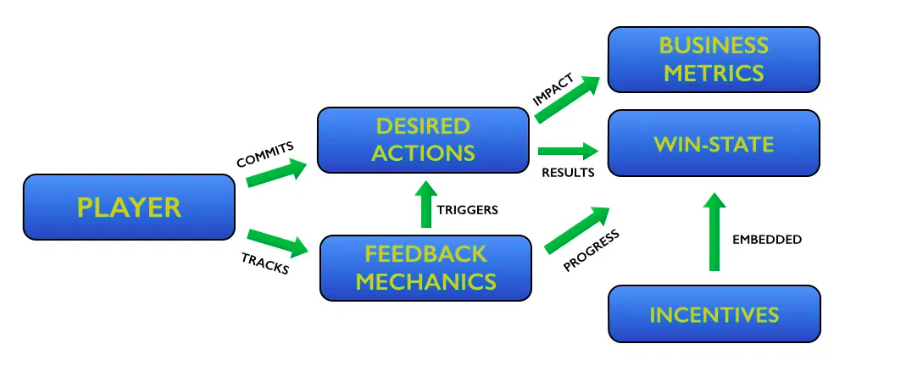
\includegraphics[width=0.6\textwidth]{images/Octalysis_strategy_dashboard.png}
    \end{center}
    These come together to form the Octalysis Strategy Dashboard. Without understanding the business metrics, the users, and the desired actions, it is very difficult to see how effective a gamified design fulfills its objective.''
\end{itemize}

\subsection{Define Business Metrics}
\begin{itemize}
    \item The list that comes from defining the business metrics, ordered by the importance, ''is based on quantifiable metrics for what creates a successful website, and less on my social and personal aspirations. Also, the ones on top are final metrics that would make a project successful, while the ones on the bottom are more of a ''means-to-an-end'' type of metrics.''
    \item ''On every interface, you will realize that you can improve many different Business Metrics, but you can only optimize for one Business Metric with the limited real-estate and user attention span. As a rule of thumb, the question to ask is, if my top three Business Metrics are doing amazingly well, while the other Business Metrics are doing modestly, would this project still be successful.''
    \item ''The Business Metrics then become the Game Objective. If these quantifiable numbers go up, then the gamification campaign is successful. If these metrics do not go up, then the gamification campaign is a failure.''
\end{itemize}

\subsection{Define user Types}
\begin{itemize}
    \item ''The next step is to define who are my target Users, which ultimately become Players in the system if the gamified designs work.''
\end{itemize}

\subsection{Define Desired Actions}
\begin{itemize}
    \item ''The next step is to define the Desired Actions for the Users, which become Win-States once they commit to the actions. This is where we lay out all the little actions and steps that we want users to take in chronological order as part of a player journey.''
    \item \textbf{Discovery Phase Desired Actions}
    \item \textbf{Onboarding Phase Desired Actions}
    \item \textbf{Scaffolding Phase Desired Actions}
\end{itemize}

\subsection{Endgame Phase Desired Actions}
\begin{itemize}
    \item ''Every designed element needs to motivate users towards these Desired Actions. If it does not, the element is a distraction and should be thrown away. Every Desired Action, when committed, leads to a Win-State.''
\end{itemize}

\subsection{Define Feedback Mechanics}
\begin{itemize}
    \item ''Feedback Mechanics are information delivery mechanisms that communicate to the user that their actions are meaningful, It allows them to track their progress towards the Win-State, feel the urgency of time, understand the unpredictable nature of the experience, and more. All Feedback Mechanics should become Triggers that promote the Desired Actions further, or else it should not be there.''
    \item ''The first step to understand possible Feedback Mechanics is to define mediums of interaction and communication. These are all the places I am able to actually plant these Feedback Mechanics as well as Triggers.''
    \item ''The second step is to figure out what Feedback Mechanics I can insert into the site. This is what most people think about when they think ''Gamification Design.'' These are the elements that allow communication of the 8 Core Drives that motivate behavior.''
\end{itemize}

\subsection{Incentives and Reward}
\begin{itemize}
    \item ''The last item to define in the Octalysis Strategy Dashboard is Rewards, which is what the experience designer can give users when they commit the Desired Actions and arrive at the Win-State.''
\end{itemize}

\subsection{Level 1 Octalysis Ideation Process}
\begin{itemize}
    \item ''Once the Octalysis Strategy Dashboard is fully defined, the next step is to go through the 8 Core Drives and come up with new ideas that appeal to people's 8 Core Drives toward the Desired Actions.''
\end{itemize}

\subsection{Repeating the Octalysis Process}
\begin{itemize}
    \item ''Once you go through the 8 Core Drives, don't stop there. Do it again. More sophisticated ideas will often flow out.''
\end{itemize}

\subsection{Summary of Level 1 Octalysis in Action}
\begin{itemize}
    \item ''When designing, it's great when lots of ideas go into the top of a brainstorming funnel. However, it is usually a bad sign when lots of ideas come out of the funnel towards implementation because it shows a lack of focus. Most companies can only implement a subset of the creative ideas in a timely manner.''
\end{itemize}




%\printbibliography
\end{document}
